\documentclass[11pt,a4paper,dvipsnames]{article}
\usepackage[deliverable]{IOHKCoverPage}


\usepackage[margin=2.5cm]{geometry}
\usepackage{iohk}
\usepackage{microtype}
\usepackage{mathpazo} % nice fonts
\usepackage{amsmath}
\usepackage{amssymb}
\usepackage{amsthm}
\usepackage{latexsym}
\usepackage{mathtools}
\usepackage{stmaryrd}
\usepackage{extarrows}
\usepackage{slashed}
\usepackage[colon]{natbib}
\usepackage[unicode=true,pdftex,pdfa,colorlinks=true]{hyperref}
\usepackage{xcolor}
\usepackage[capitalise,noabbrev,nameinlink]{cleveref}
\usepackage{float}
\floatstyle{boxed}
\restylefloat{figure}
\usepackage{tikz}
\usepackage{booktabs}
\usepackage{enumerate}
\usepackage{paralist} %% In-para enumeration -- KH
\usepackage{enumitem} %% Enumeration args -- KH
\usepackage{fancyvrb}
\usepackage{comments}

\newcommand{\khcomment}[1]{\comment{KH}{#1}}
\newcommand{\pkcomment}[1]{\comment{PK}{#1}}

\setlength{\parindent}{0pt}


%%
%% Package `semantic` can be used for writing inference rules.
%%
\usepackage{semantic}
%% Setup for the semantic package
\setpremisesspace{20pt}

% data for Deliverable header -- added by KH from an EU H2020 project template
\DeliverableNumber{PUP-D1}
\DeliverableTitle{The Design of the Cardano Ledger with Automated Parameter Updates and Central Fund Transfers}{Design Document: Automated Updates/Fund Transfers}
\DeliverableResponsible{Formal Methods Team}
\EditorName{Andre Knispel, \IOHK}
\Authors{
   Kevin Hammond \quad \texttt{kevin.hammond@iohk.io}\\
   Philipp Kant \quad \texttt{philipp.kant@iohk.io}\\
   Andre Knispel \quad \texttt{andre.knispel@iohk.io}
   % TOOO: Order by main author - currently alphabetical
}
\DueDate{30$^{\textrm{th}}$ June 2021}
\SubmissionDate{}{}
\LeaderName{Philipp Kant, \IOHK}
\InstitutionAddress{\IOHK}
\Version{PUP-1.0.0}
\Project{Voltaire Ledger}
\DisseminationDR

\begin{document}

\hypersetup{
  pdftitle={Design of the Cardano Ledger with Automated Parameter Updates},
  breaklinks=true,
  bookmarks=true,
  colorlinks=false,
  linkcolor={blue},
  citecolor={blue},
  urlcolor={blue},
  linkbordercolor={white},
  citebordercolor={white},
  urlbordercolor={white}
}


\floatstyle{boxed}
\restylefloat{figure}
\cleardoublepage
\renewcommand{\thepage}{\arabic{page}}
\setcounter{page}{1}

\title{Design of the Cardano Ledger with Automated Parameter Updates and Central Fund Transfers}

\author{
   Kevin Hammond \\ {\small \texttt{kevin.hammond@iohk.io}} \\
   Philipp Kant \\ {\small \texttt{philipp.kant@iohk.io}} \\
   Andre Knispel \\ {\small \texttt{andre.knispel@iohk.io}} \\
   }

\date{}

\maketitle

\begin{abstract}
  This document outlines the design of the mechanisms that are needed to support
  automated parameter updates and central funds transfers (collectively PUP).  The PUP mechanism enables a key part of the Cardano governance structure by
  eliminating the use of genesis keys or delegates to control the operation of the Cardano blockchain.  This enables decentralised governance of the blockchain.
  The overall governance process includes both
  off-chain and on-chain components.  This design document is concerned primarily with the on-chain component, but also references the corresponding off-chain
  process, and discusses how the two components interact to ensure decentralised governance.  It covers all parts of the on-chain process including proposal submission,
  vote delegation, on-chain voting/endorsement and automated enactment of proposals.
\end{abstract}

\section*{List of Contributors}
\label{acknowledgements}

\begin{changelog}
\change{2021-02-16}{Kevin Hammond}{FM (IOHK)}{Initial version. }
\change{2021-02-17}{Kevin Hammond}{FM (IOHK)}{Description of goals and submission process.}
\change{2021-02-19}{Kevin Hammond}{FM (IOHK)}{Groups involved.  Vote delegation.}
\change{2021-02-19}{Kevin Hammond}{FM (IOHK)}{Added various outline sections.  Voting, sidechains, short Priviledge comparison.}
\change{2021-02-22}{Kevin Hammond}{FM (IOHK)}{Added workflows, plus textual improvements.}
\change{2021-02-25}{Kevin Hammond}{FM (IOHK)}{Added transition process, updated diagrams, described endorsement and enactment, cleaned up text.}
\change{2021-03-01}{Kevin Hammond}{FM (IOHK)}{Reviewed and updated text.  Added missing diagram, section on transition.}
\change{2021-03-03}{Kevin Hammond}{FM (IOHK)}{Added appendix on user experience.}
\change{2021-03-05}{Kevin Hammond}{FM (IOHK)}{Revised and tidied.  Added address structure and other diagrams.  Checked against delegation design document.}
\change{2021-03-10}{Kevin Hammond}{FM (IOHK)}{Clarified automated endorsement.  Decision needs to be taken on whether endorsement is stake-based or block-based.}
\change{2021-03-12}{Kevin Hammond}{FM (IOHK)}{Added appendix on protocol parameters.  Updated text.}
\change{2021-03-12}{Kevin Hammond}{FM (IOHK)}{Incorporated initial feedback from Andre and Philipp.}
\change{2021-03-15}{Kevin Hammond}{FM (IOHK)}{Added Section on Design Notes to record discussion.}
\change{2021-04-01}{Kevin Hammond}{FM (IOHK)}{Added Appendix on Native Token Governance}
\change{2021-04-01}{Kevin Hammond}{FM (IOHK)}{Added Appendix on Expert Ballots}
\change{2021-04-09}{Kevin Hammond}{FM (IOHK)}{Added Section on Differentiated Submission Groups}
\end{changelog}



%% Using \include, so these can be omitted in the final version
\pagebreak
\section*{To Do}

\newcounter{todo}
\begin{tabular}{||p{0.25in}|p{5.7in}||}
  \hline \hline \stepcounter{todo}  \thetodo &
  Consider transaction costs for voting -- will this be off-putting?
  \\ \hline \stepcounter{todo} \thetodo &
  Confirm sizes of items in certificates
  \\ \hline \stepcounter{todo} \thetodo &
  Confirm required stability window deadlines
  \\ \hline \stepcounter{todo} \thetodo &
  Side-chain integration needs to be fleshed out, if required
  \\ \hline \stepcounter{todo} \thetodo &
  Efficiency needs to be properly evaluated
  \\ \hline \stepcounter{todo} \thetodo &
  A security audit needs to be done, and any issues addressed
  \\ \hline \hline \stepcounter{todo}  \thetodo &
  Consider the composition and election of the submitter group
  \\ \hline \stepcounter{todo} \thetodo &
  Take legal advice where needed
  \\ \hline \stepcounter{todo} \thetodo &
  Decide whether exchanges should be permitted to vote -- if not, token locking may be needed to prevent that, BUT that will impact participation levels
  \\ \hline \stepcounter{todo} \thetodo &
  Many specific details need to be discussed, and solutions found
  \\ \hline \hline
\end{tabular}

%% Done
%  Votes can never be lost
%  Check terminology: addresses, certificates, keys
%   Change the diagrams to show that voting and endorsement can be independent

\pagebreak


\pagebreak
\section*{Design Notes}

This section covers some key design issues that have been discussed, and explains how they have been resolved.

\newcounter{issue}

\stepcounter{issue}
\subsection*{Issue \theissue{}: Should votes be based purely on stake?}

\subsubsection*{Description of Issue.}

Basing voting power purely on the stake that is held potentially disenfranchises some groups that have a
significant investment in the ecosystem.  While block production relies on \emph{Proof of Stake},
it is not necessarily clear that voting should follow the same principle.  There c

\subsubsection*{Alternative Solutions.}

\begin{enumerate}
\item
  \emph{Votes are based on stake.}  This is the obvious solution.
\item
  \emph{Votes are based on fees paid.}  This enfranchises the users of the system.
\item
  \emph{Votes are based on transaction volume.}  This also enfranchises users.
\item
  \emph{Votes are based on identity.}  This creates a more democratic system.
\item
  \emph{Hybrid.}  For example, part of the vote is based on stake, part on the fees paid, in some pre-determined proportion.
\end{enumerate}

\subsubsection*{Chosen Resolution.}

We will use the obvious solution (Option 1: stake-derived voting).  This fits
with the existing stake delegation design, so simplifying the design and
implementation, and minimising the number of new mechanisms that are required.
It also simplifies security concerns -- it is not possible for a cabal to take
over the blockchain, without first gaining the authorisation of the majority of
the held stake.

\stepcounter{issue}
\subsection*{Issue \theissue{}.}

\subsubsection*{Description of Issue.}

\subsubsection*{Alternative Solutions.}

\subsubsection*{Chosen Resolution.}

\pagebreak


\tableofcontents

\clearpage
\listoffigures

\clearpage
\section{Introduction}

The aim of this design is to eliminate the use of the genesis keys (or delegates) within the formal ledger rules.  This will enable
decentralised governance of the blockchain protocol by supporting automated submission and enactment of proposals (PUP).
The process is designed to meet current and future national and international regulatory concerns by removing control of the blockchain protocol
from a small centralised group of actors.

There are three places where genesis keys are currently used.


\begin{itemize}
\item
  \textbf{Parameter Updates:}
  Any updatable protocol parameter may be changed.  Multiple parameters may be changed as part of a single update proposal.
\item
  \textbf{Protocol Version Changes:}
  A change may be made to a major or minor protocol version (a ``hard fork'').  The change must be accompanied by upgrades to
  the software that is being used by block producing nodes (``stake pools''), and acknowledged by sufficient pools upgrading to the new software version.
\item
  \textbf{Transfers from/to Reserves/Treasury:}
  A funds transfer may be made directly from eiher the reserves or treasury pots to a nomrmal address, between the reserves and treasury pots (in either direction), or from a normal address to the treasury pot.  This is referred to in the existing Cardano documentation as an ``MIR'' transfer (Move Instantaneous Rewards).
\end{itemize}

All of these issues must be devolved to a decentralised governance process.

\subsection{Outline Governance Process}

The proposed governance process involves both off-chain and on-chain components.

\begin{enumerate}
\item
  \textbf{Off-Chain:}
  An issue is discussed off-chain.  A vote is taken on a specific proposal using the Catalyst system.  The proposal must be sufficiently unambiguous that its intention is clear, and must include dates by which the proposal is to be submitted and enacted on chain.
\item
  \textbf{On-Chain:}
  A formal proposal is constructed that captures the intention of the off-chain proposal.  It is submitted, verified, and then enacted on-chain.  The proposal will specify the date at which it will be enacted if it is
  properly accepted and endorsed.
\end{enumerate}


The outline process for enacting a proposal is shown in Figure~\ref{fig:workflows}.   The process is split into two main parts: the initial off-chain process, which is expected to be largely manual; and the second, on-chain process, which will largely be
automated.  Only the latter needs to be captured by formal ledger rules.  In order to establish confidence in the governance process,
it is necessary to link the off-chain and on-chain processes.

\begin{figure}
  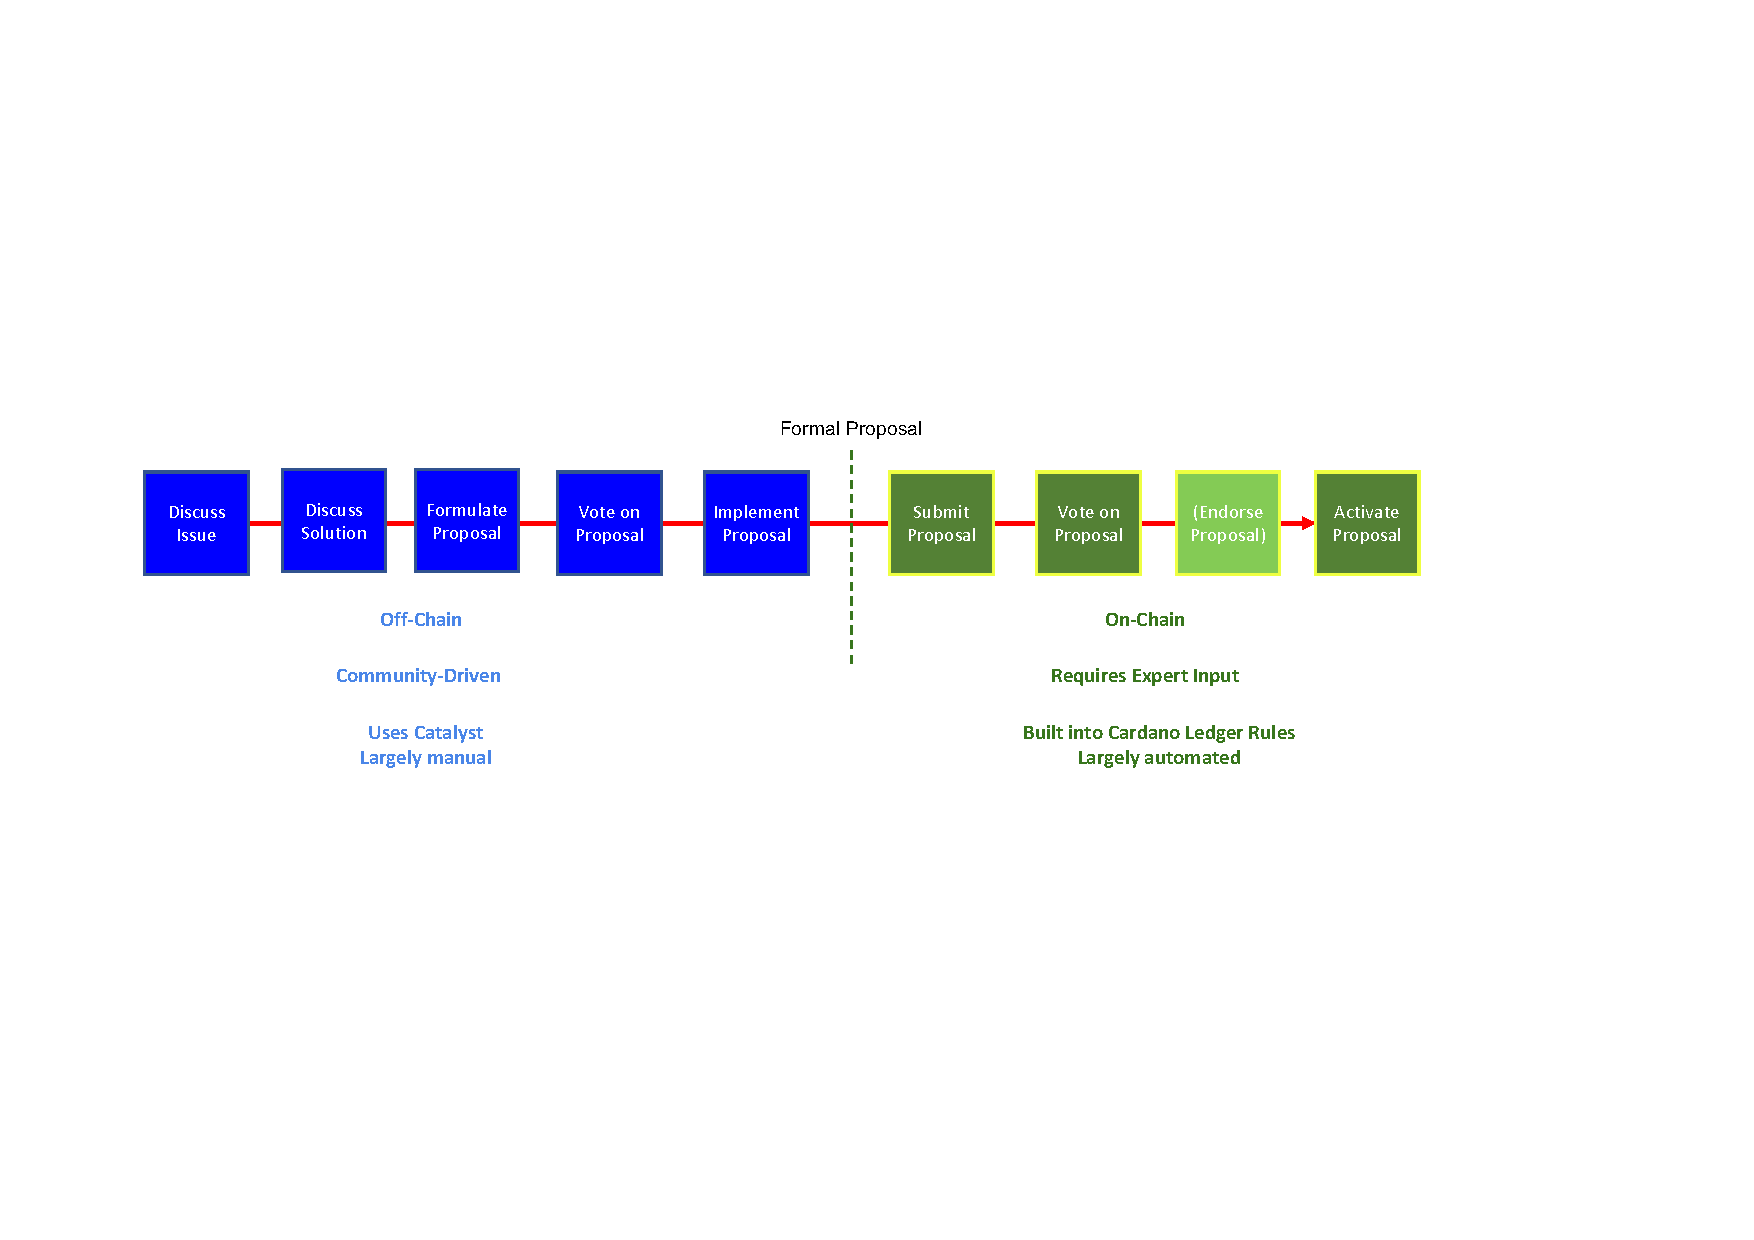
\includegraphics[trim=30 200 100 100,clip,width=\textwidth]{StoryBoard}
  \caption{Outline Process: Ideas are discussed off-chain and voted on using the Catalyst mechanism.  Successful proposals are implemented, and then submitted for on-chain voting and enactment.}
\label{fig:workflows}
\end{figure}


\newpage
\subsection{Off-Chain Process}

The off-chain process involves five key stages:

\begin{enumerate}
\item
  \textbf{Discussion.}  An issue is discussed.  This may be either formal or informal discussion, using a mechanism such as IdeaScale, a community forum such as a TeleGram channel or the Cardano Forum,
  or any other appropriate mechanism.
\item
  \textbf{Ideation.}  A concrete proposal that addresses the issue is formulated by an interested party.
\item
  \textbf{Submission.}  A proposal is submitted for voting.  The submission of proposals must follow the defined process, and may be restricted in some way.
\item
  \textbf{Voting.}  Voters may vote on whether a proposal should be progressed to implementation, requires amendment etc.  Outline or exact deadlines should be agreed as part of this process.
\item
  \textbf{Implementation.}  Accepted proposals are implemented.  For a simple proposal (eg a change to an updatable parameter), this may be as simple as capturing the intentions of the original proposal in a corresponding JSON file.
  Proposals to change protocol versions may involve significant software development, and therefore need to be funded by the Catalyst fund or some other means.
\end{enumerate}

Each of these off-chain stages may follow formally defined processes, and may be partially automated.  Generally, they will be driven by convention and rules.  A detailed governance structure is necessary to ensure that necessary business can
be transacted in an efficient and effective way, without risking loss of control to a small non-representative group, and so negating the purpose of decentralised governance.
The processes and structures may evolve over time.  Some of the issues are discussed in Appendix~\ref{sect:off-chain}.


\newpage
\subsection{On-Chain Process}

Once a proposal has been implemented in the required form, it may be submitted for enactment on-chain.  The on-chain process involves four key stages that are fully automated.  Extreme care needs to be taken with these processes,
since it may not always be possible to stop or reverse actions once they are initiated.

\begin{enumerate}
\item
  \textbf{Submission.}  A formal proposal is submitted on-chain by one of a group of submitters.  The proposal must be in the agreed format, and must include deadlines for voting, endorsement and enactment.
\item
  \textbf{Voting.}  The proposal is voted on and the votes are tallied.  If sufficient votes are obtained by the stated deadline, then the proposal is approved for enactment.
\item
  \textbf{Endorsement.}  If the proposal involves a change to the protocol, then stake pool operators must upgrade their nodes to the correct version.  This will signal their readiness to run the new protocol.
  Assuming that sufficient endorsement is obtained by the deadline, then the proposal is endorsed for enactment.
\item
  \textbf{Enactment.}  Proposals that have been approved (and endorsed, if necessary) are processed fully automatically at the corresponding epoch boundary.
\end{enumerate}

\newpage
\subsection{Key Stakeholder Groups}

A number of stakeholder groups are involved in the governance process.  The key ones are:

\begin{itemize}
\item
  \textbf{Normal Ada Holders:}
  Normal Ada holders are invested in the Cardano ecosystem in financial and other ways.
   In order to ensure fully decentralised governance, the goal of the PUP design is that normal Ada holders should have the ultimate governance power. They may, however, choose to delegate this to specialists when dealing with more technical issues, for example.
%  This ensures fully decentralised governance.
  \item
  \textbf{Stake Pool Operators:}
  Stake pool operators have the responsibility for maintaining the Cardano network.  They are heavily invested in the Cardano ecosystem through the commitment of their time, money and other resources.
  In addition to other voting rights, they need to maintain software compatibility with the latest version of the Cardano blockchain protocol.
  \item
  \textbf{End-Users:}
  These are individuals or organisations who use the Cardano blockchain to process transactions etc.  They may hold minimal ada, perhaps only on a transient basis.
  This will give them limited or no governance rights.  Their needs should, however, be considered when changes are made to protocol parameters.
  \item
  \textbf{Exchanges and other Proxy Ada Holders:}
  Exchanges and similar organisations hold Ada on behalf of other parties.  It is important from both a regulatory and a technical perspective that they do not hold excessive
  power, since this will work against the requirements of decentralisation.  They require a safe, secure and robust blockchain so that they may operate successfully on
  behalf of their clients.
\end{itemize}

The network should be able to evolve in a way that meets the best long-term needs of all these stakeholders, while maintaining the integrity, stability and longevity of
the Cardano blockchain.

\section{Detailed Design Goals}
\label{sect:goals}

The primary goals of this design are:

\begin{itemize}
\item
  \textbf{Decentralised Governance:}
  Support a decentralised governance mechanism for Cardano.
\item
  \textbf{Genesis Key Retirement:}
  Remove the dependence of the Cardano blockchain on a small set of genesis keys/delegates.
\item
  \textbf{Security:}
  Maintain the security of the Cardano network.
\item
  \textbf{Progress:}
  Ensure that the blockchain protocol can evolve in the necessary way.
\item
  \textbf{Smooth Transition:}
  Evolve smoothly from the current federated governance
\end{itemize}

Where these goals conflict, it is, of course, absolutely essential to maintain the security of the network.  Maintaining progress/enabling
evolution is also important, since otherwise governance decisions will be ineffectual/not enacted.

\pagebreak
\subsection{Overall Governance Goals}

The primary reason for decentralisation is to ensure long-term compliance with emergent and evolving international financial regulations.
Secondary reasons include improved community engagement, alignment of decision-making authority with increased responsibility for maintaining the blockchain,
ensuring the long term stability of the Cardano blockchain.  Decentralisation means that decisions about the operation and evolution of the blockchain
should be taken collectively by representive groups of stakeholders.
%
Achieving these goals requires that:

\begin{itemize}
\item
  The governance process is transparent -- the progress of decisions can be monitored and any deviations are properly explained to stakeholders.
\item
  All opinions are considered.
\item
  Control of the blockchain rests with those who have the greatest direct stake in the operation of the blockchain either as holders of ada or as maintainers of the blockchain.
\item
  Control of the blockchain is not unduly concentrated -- small, unrepresentative groups of powerful individuals should not be able to take over the operation
  of the blockchain.
\item
  The blockchain is robust to change -- it should be possible to recover from an incorrect governance decision, and any changes that are implemented will not expose the blockchain to attack.
\item
  The mechanisms that are implemented will properly incentivise stakeholders to take decisions that are in the best long-term interest of the blockchain, as well as in their own long-term interest.
\item
  There are checks and balances to ensure that technical knowledge and advice is properly considered as part of the decision making and implementation process.
  This is especially important where there are security concerns.
\item
  There is traceable continuity in the blockchain -- that is, there is an on-chain record of all the changes that are made, including the outcomes of on-chain voting, endorsement, and proposal enactment.
\item
  The transitional path to decentralised governance is clearly identified and explained, with clear steps and gates to achieving the required level of decentralisation.
\end{itemize}


It is, of course, not necessary (or probably even sensible) for every aspect of
the process to be \emph{fully decentralised}, only that
\begin{inparaenum}
\item
  the ultimate \emph{control} of
the blockchain is decentralised to the extent that is required for effective
governance, and
\item
  decentralised governance decisions are \emph{enacted} faithfully and in the
  long-term interest of the blockchain.
\end{inparaenum}
In particular, the process must not exclude those who
are less technically expert, but must properly consider technical concerns.

\subsection{Off-Chain Requirements}

There are many legitimate ways to meet the off-chain governance requirements. Appendix~\ref{sect:off-chain} considers some of the issues
that are involved.  Since this document focuses primarily on the on-chain technical design requirements, off-chain requirements will not be covered
in detail here.

\pagebreak
\subsection{On-Chain Requirements}

On-chain requirements may be split into mandatory and optional requirements.

\paragraph{Mandatory Requirements.}  The on-chain mechanism must:

\begin{itemize}
\item
  allow changes to be made to any updatable protocol parameter, in any legal way;
\item
  allow major/minor protocol versions to be upgraded;
\item
  allow the fulfilment of all kinds of central funds transfers;
\item
  not require the use of genesis keys or genesis key delegates in any part of the protocol;
\item
  allow separate per-proposal deadlines to be set for voting and endorsement;
\item
  ensure that deadlines are reasonable;
\item
  allow an epoch to be chosen for enactment of a proposal;
% \item
%   be able to faithfully enact the governance decisions that have been taken off-chain.
\item
  be secure;
\item
  be efficient;
\item
  meet the Cardano blockchain stability window requirements;
\item
  allow delegation of voting rights from ada holders to a dedicated group;
\item
  assign voting and endorsement rights in proportion to the amount of ada that is controlled;
\item
  where the proposal changes the protocol version, check that sufficient stake pools have upgraded to a compatible software version;
\item
  prevent denial-of-service attacks by limiting the proposal submission rate;
\item
  automatically enact proposals at the stated epoch boundary, provided that the necessary voting and endorsement thresholds have both been met.
\end{itemize}

\paragraph{Optional Requirements.}  In addition, the on-chain mechanism should:

\begin{itemize}
\item
  allow multiple proposals to be in-flight and enacted in a single epoch;
\item
  resolve conflicts between proposals automatically (e.g. using temporal ordering, or some other consistent and predictable mechanism);
\item
  (perhaps, allow different thresholds to be set for different kinds of proposal);
\item
  as far as possible, be consistent with the existing manual update and MIR mechanisms.
\end{itemize}

\section{Main Groups Involved}

We can identify a number of distinct groups that may be involved in proposal submission, discussion and enactment.

\begin{tabular}{||l|l|l||}
  \hline \hline
  \textbf{Group} & \textbf{How Involved} & \textbf{On-/Off-Chain?}\\
  \hline
  General Ada Holders  & Make new informal proposals. & Both \\
                       & Discuss and vote on proposals off-chain. & \\
  			               & Delegate on-chain voting rights. & \\
  \hline
  Executive Team  & Prioritise proposals. & Off-chain \\
                       & Manage off-chain votes. & \\
                       & Manage proposal discussion. & \\
  			               & Ensure that proposals are implemented. & \\
  			               & Ensure that proposals are submitted on-chain. & \\
  \hline
  Security Experts			       & Advise on Security Aspects of proposals. & Off-chain \\
                               & Track security issues and suggest fixes. & \\
  \hline
  Other Expert Groups			       & Provide feedback on proposals. & Off-chain \\
  \hline
  Proposal Editors			   & Ensure that proposals are documented & Off-chain \\
                     & in the required way. &  \\
  \hline
  Proposal Implementors			   & Produce formal proposals/software. & Off-chain\\
  \hline
  Submitters				   & Submit formal proposals on-chain. & On-chain \\
  \hline
  Delegates				   & Vote on acceptance of on-chain proposals. & On-chain \\
  \hline
  Endorsers			   & Endorse readiness for protocol version upgrade. & On-chain\\
  \hline
  Electors			       & Nominate submitters. & Either \\
  \hline \hline
\end{tabular}

\subsection{General Ada Holdera (Off-Chain and On-Chain)}

General Ada holders may make informal proposals and discuss them using an off-chain mechanism.  They vote on the acceptance of these proposals
either on-chain or off-chain, in proportion to the ada that they hold.  They may delegate their stake for voting purposes to on-chain representatives,
who will vote on their behalf for or against submitted proposals.  This vote delegation may be changed at any time.

\subsection{Executive Team (Off-Chain)}

The Executive Team is responsible for managing proposals, prioritising them for discussion and voting, monitoring the voting process and the
voting outcome, ensuring that the proposal is properly implemented and submitted on-chain, and reporting back on proposal enactment.
It is also responsible for ensuring that the correct process is followed for the type of proposal.  It may be possible to automate part or all of this process.

\subsection{Security Experts (Off-Chain)}

Security Experts evaluate proposals, provide advice on possible attack vectors, and suggest improvements to mitigate security risks.
Their input may not be necessary on some simple parameter changes, but is always necessary for protocol version changes.
They may also evaluate security threats and may, in extremis, produce proposals that bypass some of the usual governance processes
(eg where open discussion could lead to a major risk of loss to the blockchain).

\subsection{Other Expert Groups (Off-Chain)}

Other Expert Groups may be called on to provide advice or reports to inform general ada holders or other groups that are involved in the
governance process.  This could include performance issues, technical blockchain expertise, economic advice, advice on implementation etc.

\subsection{Proposal Editors (Off-Chain)}

Proposal Editors\footnote{Currently CIP Editors, where CIP stands for Cardano Improvement Proposal.} ensure that proposals are documented correctly, and that they are recorded in the
permanent repository.
This provides a persistent record of the rationale for each proposal, and allows traceability between informal off-chain
proposals and the formal on-chain proposal.  This process may include providing hashes or other information to support traceability.

\subsection{Proposal Implementors (Off-Chain)}

Proposal Implementors transform accepted proposals that have been voted on by ada holders into formal proposals that can be submitted on chain.
They are responsible for providing necessary documentation, and for compliance with the required processes.  This may include producing an acceptable formal proposal
\footnote{CIP}
and meeting any necessary verification/traceability requirements.  For simple parameter updates or funds transfers, implementation may be in the form of a single JSON
file that fully describes the proposal. Protocol version upgrades will also require the corresponding software implementation.

\subsection{Submitters (On-Chain)}

Submitters are permitted to submit proposals on-chain.  Each proposal must be signed by a quorum of submitters, who verify the submitted
proposal, checking that it is in the correct format, conforms to the original proposal, and meets other process requirements.
Submitters are appointed by endorsers.  Depending on the governance design, the submitter group might be restricted to a few members,
be an elected or appointed group, be limited by ada holding, or be limited to endorsers, delegates or another group.

\subsection{Delegates (On-Chain)}

Delegates vote on whether an on-chain proposal should proceed.  The weight of
their vote is in proportion to the stake that has been delegated to them by
normal ada holders, including themselves.  They are expected to be responsible
experts, to represent those who have chosen to delegate vote to them, and will
be respected community members.  Although in many cases delegates may also be
stake pool operators, the separation of vote delegation from delegation for
block production separates politics from economics.  Ada holders may choose to
delegate ada to good block producers in an apolitical way, and to support
delegates that represent their political opinions without considering their abilities as
block producers.  Delegates must track any discussions and ensure that the proposals meet the required
security and other concerns.

\subsection{Endorsers (On-Chain, May not be needed)}

The role of an endorser is to confirm that they are ready to upgrade to a new
version of the Cardano protocol.  All stake pools are endorsers.  In line with
the principle of proof-of-stake, the weight of their endorsement is proportional
to the stake that they control.  In order to ensure that the blockchain will
make progress, and that the main chain will not split, a sufficient stake
threshold of endorsement is required for a proposal to be enacted.

\subsection{Electors (Off-chain or On-Chain)}

Electors determine who belongs to the submitter group.  The composition of this group is to be determined.  It might be formed by direct election off-chain, by
nomination from an agreed group, by submission of an on-chain proposal.  In some systems, it may even be unnecessary.

\begin{figure}
  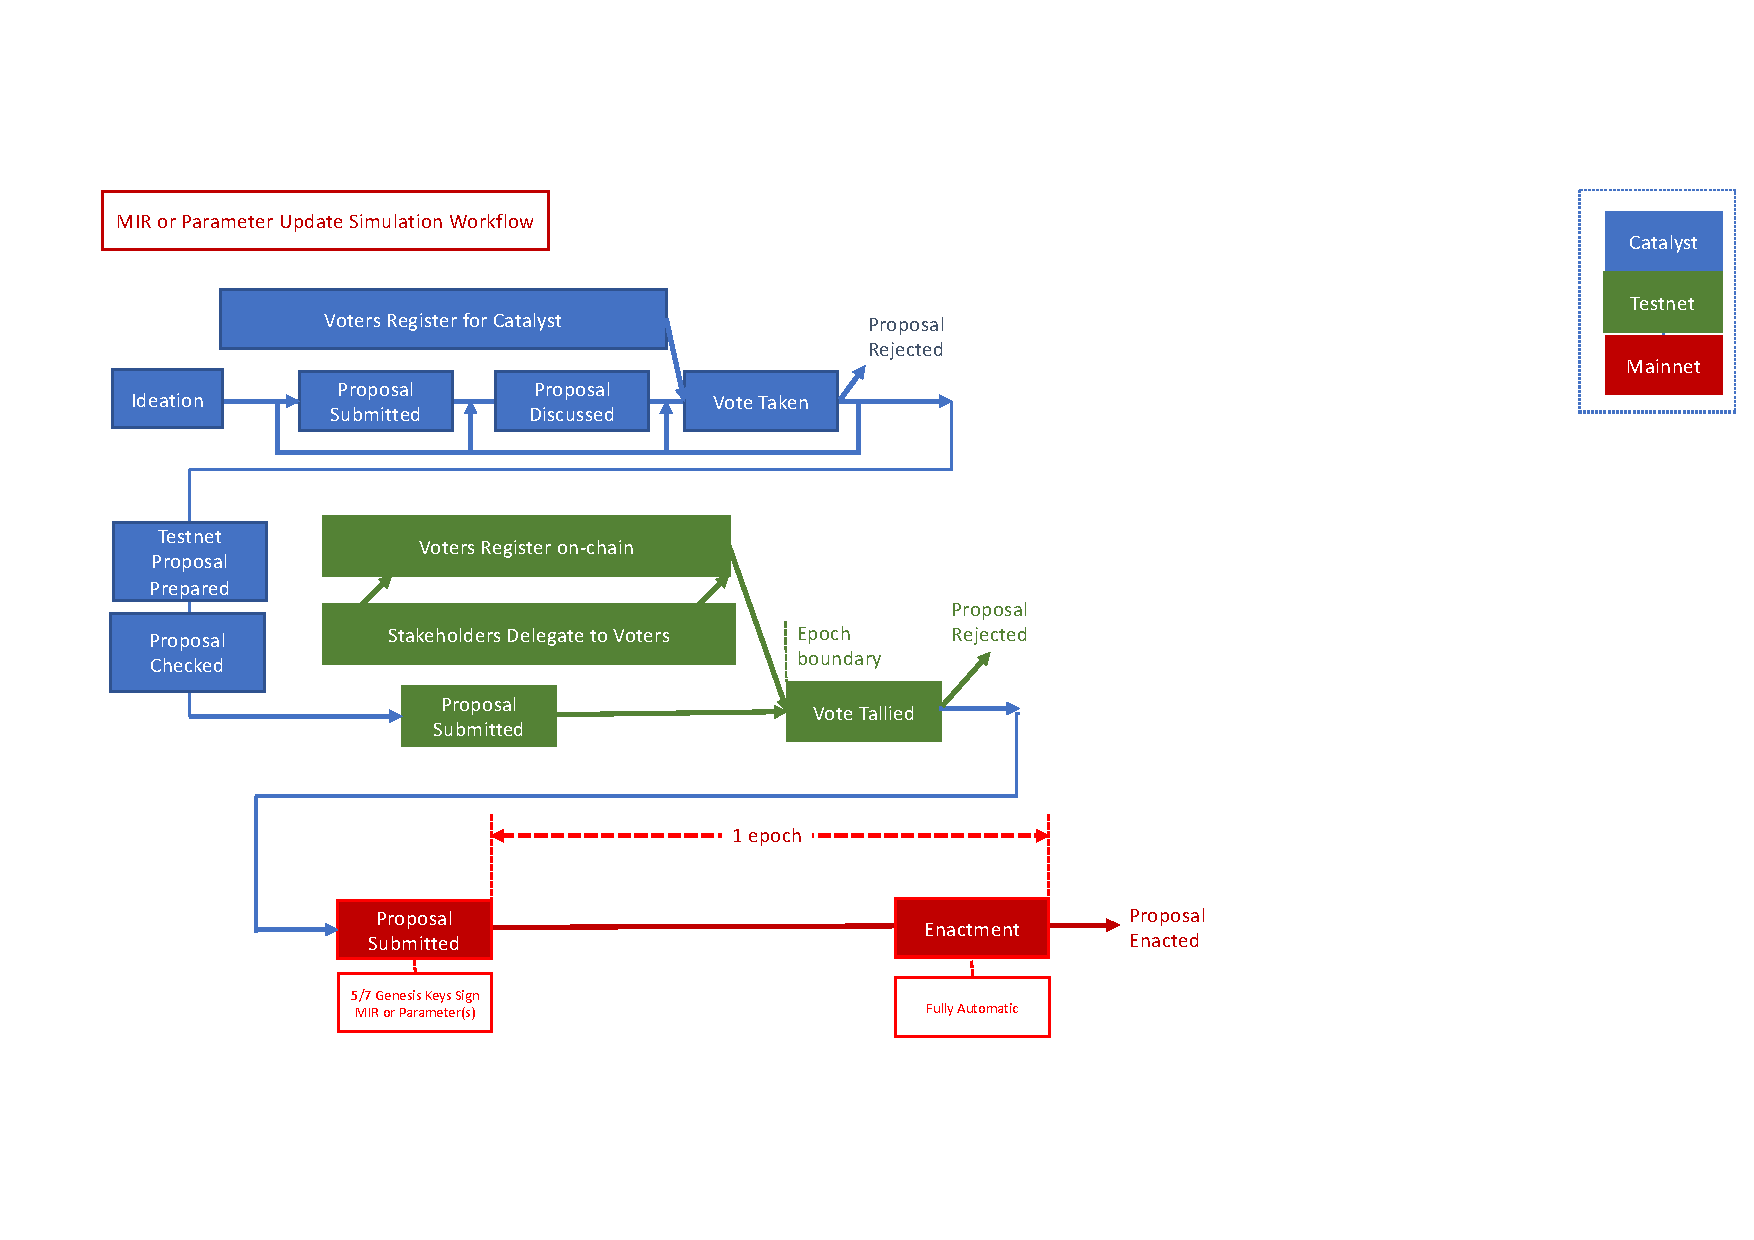
\includegraphics[trim=0 90 0 80,clip,width=\textwidth]{Workflow1}
  \caption{Example Workflow: Funds Transfer (MIR) or Simple Parameter Value Update}
  \label{fig:workflow-mir}
\end{figure}

\section{Example Workflows}
\label{sec:workflows}

Figures~\ref{fig:workflow-mir}-\ref{fig:workflow-hf} show outline workflows for
typical use cases.  Figure~\ref{fig:workflow-mir} shows the workflow that is
involved in submitting either a proposal to transfer funds, or to change the
value of an updatable protocol parameter.  Figure \ref{fig:workflow-hf} shows
the corresponding workflow for a protocol version change (``hard fork'').

\paragraph{Parameter Updates and Funds Transfers.}  Parameter update and funds transfer proposals involve three main stages:
proposal submission, on-chain voting, and proposal enactment.  In the workflow that is described
here, proposal preparation, proposal submission, delegate registration,
vote delegation and voting involve manual steps, but stake snapshots, vote tallying
and enactment are fully automatic.  Stake snapshots are taken at each epoch boundary.
These govern the weight of each vote delegation during the upcoming epoch.
%
Delegates may register at any time.  Ada holders may delegate to any registered delegate.
Delegates may choose to vote on any active proposal prior to the specified vote deadline.
Following the deadline, all votes are tallied.  If a proposal does not receive sufficient vote, then
it will be automatically rejected.  Otherwise, it is automatically accepted, and passed on for
automatic enactment.

\begin{figure}
  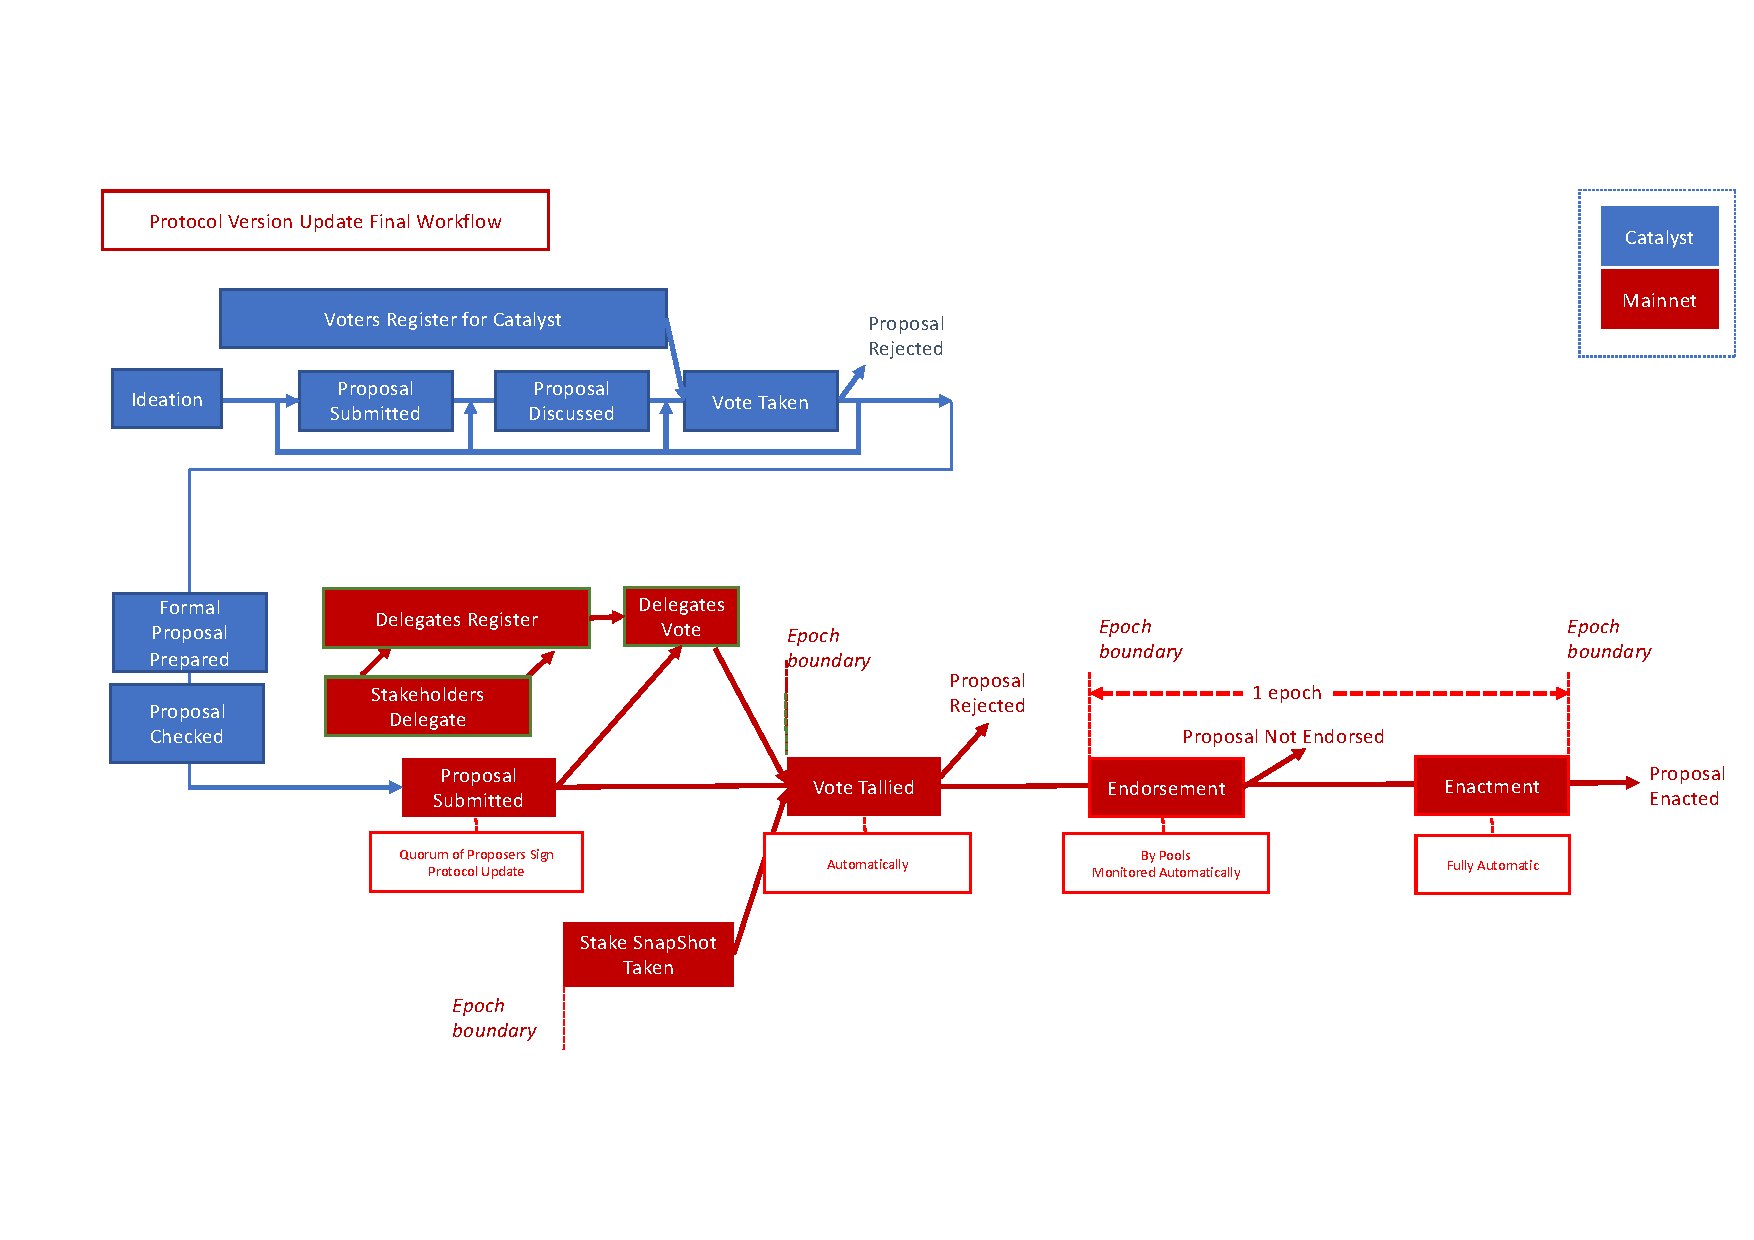
\includegraphics[trim=0 90 0 80,clip,width=\textwidth]{Workflow2}
  \caption{Example Workflow: Protocol Version Update (Hard Fork)}
  \label{fig:workflow-hf}
\end{figure}

\paragraph{Protocol Version Updates (Hard Forks).}  These follow the process described above,
except that the proposal must also be \emph{endorsed} by sufficient block-producing stake
(where endorsement indicates the readiness of the stake pool operator to upgrade to the new protocol version).
The same process applies to both major and minor protocol version upgrades.
The deadline for endorsement must be given in the original proposal submission.
In order to ensure the stability of the chain, endorsement must happen sufficiently before the update takes
effect.  This has been fixed at $XX$ slots prior to the epoch where the proposed is enacted.
If a proposal does not pass the endorsement threshold then it will be rejected at this point, otherwise it will be
passed on for automatic enactment.  It is anticipated that endorsement will be through manual confirmation by each stake pool operator, though it would be possible
to automate this by monitoring software versions.\khcomment{Jared has defined an automated process.}
While the endorsement deadline will usually be after the voting deadline, this is not technically necessary, and the deadlines could
in principle be contemporaneous, or even reversed.

\paragraph{Rejected Proposals.}   Once it has been rejected, a proposal is never enacted on-chain.
An equivalent proposal may, however, be submitted, in which case the new proposal must go through the same voting and enactment process
as the original proposal (and may, itself, be rejected).

\newpage
\section{Proposal Submission}
\label{sect:submission}

Proposals are submitted by a member of a submitter group.  They must be counter-signed by a quorum of submitter keys, where the quorum is specified by the \texttt{ProposalQuorum} parameter.
%\khcomment{Difficult question: who controls registration/de-registration of submitter keys.}\pkcomment{How about an on-chain vote by ada holders?}\khcomment{That isn't possible without extending the design, of course...  You could include this as an update proposal, of course, but who submits the proposal and how do you avoid the submitter group then vetoing changes?}\khcomment{How do we
%ensure that there are always enough submitters in existence.}\pkcomment{We should have an option to reboot this set by a vote from ada holders, in case there are not enough (active) submitters}\khcomment{The
%quorum may be a protocol parameter.}\pkcomment{with an enforced sensible range in $(0,1)$}\khcomment{Yes.  I was expecting an integer value, though.  Consider the edge case where there are only a few submitters, or awkward cases where the number of submitters changes. Do you round up or down?}  No fee is charged for proposal
%submission.\khcomment{This may need to be discussed.}
A submitter may submit any number of proposals in a single epoch.
%\khcomment{This assumes that submitters are trustworthy and will not collectively spam the blockchain.  One possible solution is to use percentage of voting stake to choose the composition of this group as a subset of the delegator group.  Doing so removes one balance in the system, however (delegates propose the business that they will vote on, so potentially creating a power bloc).}
%\pkcomment{Depending on how we accumulate the counter signatures (including all of them in the transaction with the proposal, which requires off chain coordination between the submitters, or collecting them in susequent transactions) it might also be possible for a single submitter to spam the chain}
%\khcomment{The obvious approach is to use multi-sig transactions, or similar.  That would prevent multiple proposals from spamming the chain [you might be able to resubmit the same proposal, of course].  Requiring multiple transactions would be more problematic.}
It is assumed that the submitter group acts honestly on behalf of the stakeholders, and will not act to ``spam'' the chain with proposals or to prevent progress.  Suitable governance mechanisms must also be put in place to ensure that it is not possible for an unrepresentative ``cabal'' to gain control of the blockchain.

\subsection{Format}

Each proposal has a header and a body.  % and must be signed\khcomment{Submitting may implicitly sign the proposal?}.

\paragraph{Header.} The header must include:

\begin{verbatim}
"header": {
  "linked"           : ProposalHash,
  "voteby"           : Slot,
  "votethreshold"    : Threshold,
  "endorseby"        : Optional Slot,
  "endorsethreshold" : Optional Threshold,
  "enact"            : Epoch,
  "submitter"        : KeyHash
}
\end{verbatim}% \pkcomment{Do we need \texttt{Slot}, or \texttt{Epoch}?}\khcomment{You want Slot, because that is what matters for consistent voting [I assume you want the current speed of enactment]}

The \texttt{linked} field allows the proposal to be linked with the previous off-chain or on-chain acceptance (see Appendix~\ref{sect:relating-off-and-on-chain} and Section~\ref{sect:proposalid}), so enabling a chain of approval.  The \texttt{voteby} and \texttt{endorseby} fields specify deadlines.
Votes and endorsements must be received prior to the specified slot if they are to be counted.  The endorsement deadline is only required for protocol version upgrades.
%\khcomment{Arguably, to avoid performance issues, tallying should either happen at epoch boundaries or in a separate thread.}\pkcomment{Yes, same as for calculating the stake distribution and the rewards}
To avoid performance issues, tallying must be spread over time, eg in a separate thread or using a ``pulsing'' calculation. % \pkcomment{Yes, same as for calculating the stake distribution and the rewards}
In order to avoid zombie proposals that could disrupt operations, deadlines must be set within a reasonable time period after submission (e.g. within 3 epochs).
Voting and endorsement slots and thresholds are completely independent, so a voting deadline may be set before/after/at the same time as an endorsement deadline.
Deadlines can never be set in the past.
The deadline for proposal enactment must be later than the  voting and endorsement deadlines, and account for required stability windows.
%
The \texttt{votethreshold} and \texttt{endorsethreshold} fields allow specific thresholds to be set for voting and endorsement, respectively.  This allows the type of proposal to be differentiated on a per-proposal basis
(e.g. a protocol version upgrade may require a higher vote threshold than a simple parameter change)
\footnote{Arguably, this is dangerous and standard or minimum thresholds should be set as protocol parameters.}.
%
The \texttt{enact} field specifies when the proposal is to be enacted if it is approved and endorsed.  This will always be in the future.
%
The proposal submitter must belong to the correct submitter group.  \footnote{It would be possible to support
  different groups for each kind of proposal.}

The body of the proposal is specific to the proposal type.

% \newpage
\paragraph{Parameter Update Body.}  The proposal format is identical to that used for Shelley/Allegra/Mary/Alonzo. \TODO{Check the concrete format.}  Multiple parameters may be changed in a single proposal if required.
All parameters in a proposal must comply with \emph{validity} rules both on submission and on enactment.
% Parameters are checked for validity on enactment, rather than on submission, so it is possible to submit a proposal that will change parameters following a future protocol version upgrade, for example.
% \khcomment{Consider this carefully. We do need to allow initial parameters to be set.}


\begin{verbatim}
"body": {
  "parameter n" : "new value 1",
  ...
  "parameter n" : "new value n"
}
\end{verbatim}

\paragraph{Protocol Version Upgrade Body.}  The format is slightly changed from that used for Shelley/Allegra/Mary/Alonzo.


\begin{verbatim}
"body": {
  "Major"       : Integer,
  "Minor"       : Integer,
  "Genesis"     : Hash,
  "CodeVersion" : [Hash]
}
\end{verbatim}

The major and minor protocol version numbers identify the new protocol.  The genesis parameter hashes the genesis file, so ensuring that consistent initial protocol parameters are used.
The proposal also includes a list of hashes that can be used to identify one or more reference versions of the node software that implement the new protocol (e.g. as references to a specific git commit).
Node operators are not required to use one of these versions -- any software that follows the protocol rules may be be used
\footnote{Recommended software versions could also be included in the genesis file if desired.}.
% Node software only needs to comply with the new protocol rules.  It does not need to be a specific version, for example, and we do not check a software hash.
% \khcomment{I assume that
The initial set of protocol parameters is encoded in the genesis hash.

% \khcomment{We might also need to include some hash here that can be verified by the system?} % Dealt woth

\paragraph{Central Funds Transfer Body.}  The format is also identical to that used for Shelley/Allegra/Mary/Alonzo.
A single proposal may cover multiple funds transfers.  These are enacted in the order they are encountered.
% \khcomment{There is a tradeoff here: submit many proposals that may clog up the system, or submit a few.  Even if there are fewer proposals, transaction size limits mean
% that a set of transfers (for Catalyst funds, for instance), may  need to broken down into a large number of submission.}

\begin{verbatim}
"body": {
  "from"      : "Treasury"/"Reserves",
  "to"        : Optional "Treasury"/"Reserves",
  "toAddress" : Optional Address,
  "amount"    : Nat
}
\end{verbatim}

Funds may be transferred from either the treasury or the reserves, and sent to either an address, or to the treasury/reserves.
Transfers from treasury to treasury or from reserves to reserves are not permitted.  All transfers must be for a positive amount (including zero, which might be required for accounting or automation reasons). %\pkcomment{Why do we want to allow zero here?})\khcomment{I was assuming that this might be needed for accounting or automation reasons}.
Multiple transfers may be made in a single epoch.  This allows for proper accounting, where e.g. different kinds of transfer must
be authorised by different groups.

Errors in transfers between reserves and treasury, or vice-versa, may be corrected by constructing a reverse transfer that cancels the original error.
This cannot happen for transfers to addresses.  Any errors in such transfers, must be corrected by the owner of the address, who must either explicitly transfer
the funds to reserves or treasury, or else transfer the funds to a holding account\footnote{Note that there is currently no way to transfer funds back to treasury/reserves.}
Note that ledger rules ensure that the treasury and reserves may never decrease below zero (even temporarily), so that a ``double-spending attack'' is not possible.
% \khcomment{Jared to confirm.}

\subsection{Proposal Signing}

All proposals must be signed when they are submitted.  A proposal must be counter-signed by a quorum of signatures using a signing
policy that conforms to the existing \emph{multi-sig} transaction mechanism.  This enables the use of standard transaction witnessing.
% where the quorum is a protocol parameter
The signing policy is then provided as an updatable protocol parameter.  This gives a great deal of flexibility to define and change submission policies.
To reduce the possibility of abuse, the policy must comply with a minimum quorum size, which must be hard-wired into the protocol as a non-updatable
parameter.
Note that limits on transaction size will limit the maximum quorum size (currently to around 500 signatories).


%\khcomment{The obvious approach is to use transaction witnessing and a multi-sig approach, as described here.  That implies a change to the submission process, and also that
%  the submitter group is sufficiently small to allow this (I think we calculated n+m=500, where n is the actual number and m is the required number?}
% \khcomment{Using multi-sig potentially allows policies to be defined as described above.  This simplifies the system by removing the need for a separate Elector group,
%  but is perhaps open to abuse of power?}

Note that the process described here intrinsically supports automation.  Signatories can be automated agents if desired rather than individuals.  This also allows integration into a full on-chain voting mechanism in the longer term, e.g. by adopting the PriviLedge mechanisms.  The outcome of an off-chain or on-chain vote may be to construct a signed on-chain proposal for subsequent enactment.  Ultimately, if the process is purely on-chain, then the vote outcome could be embedded as the authorisation for the proposal submission without needing to construct or maintain special submitter keys.  This would improve some aspects of security, but would mean that either: i) a proposal would need to be formalised prior to the initial voting round (which might be impractical for e.g. protocol upgrades or some forms of funds transfers); or else ii) delegates would need to confirm that the proposal that was enacted was equivalent to the one that was originally agreed.


\subsection{Proposal Identifiers}
\label{sect:proposalid}

Each proposal has a unique identifier that is used for voting, endorsement, and enactment.  It may also be used to refer to the proposal in the off-chain process (eg to provide its
status, encourage voting, etc).  At a minimum, uniqueness must be enforced between submission and enactment, but it will be simplest to have full uniqueness, since the blockchain will need to record
details of each proposal indefinitely.

There are three obvious ways to construct an identifier.

\begin{description}
\item
  [Option 1.]
  An explicit identifier that is included in the proposal submission.  This could be tied, if desired, directly to the off-chain proposal/discussion.
  Care needs to be taken to ensure uniqueness of any manually assigned proposal identifier.  This is shown above as the \texttt{proposal} field.
\item
  [Option 2.]
  The identifier is constructed by hashing the submitted proposal.  This allows proposals to be identified before submission as well as during voting and enactment.  This property may be
  useful to connect off-chain and on-chain mechanisms for example.  \emph{Collision resistance} is required for the hash. % \khcomment{Confirm this.}  Confirmed.
\item
  [Option 3.]
  The transaction identifier is used to identify the proposal.  This has the advantage that it is already available on-chain, and is guaranteed to be unique.  However, it cannot be
  referred to prior to on-chain proposal submission.  Moreover, the transaction identifier cannot be relied on until the chain is stable, potentially creating confusion/an opportunity for attack.  \emph{Security cincerns therefore rule this option out.}
\end{description}

It is proposed to use Option 2, but to also include an explicit reference.  This allows
the formal proposal to be linked to off-chain or on-chain discussions and/or votes.
The reference does necessarily not need to be unique -- a single discussion or outline vote could
lead to multiple on-chain proposals.

\subsection{Proposal Validity Rules}
\label{sect:validity}

A proposal is checked for validity at two points:
\begin{enumerate}
\item
  on submission;
\item
  on enactment.
\end{enumerate}

Invalid proposals are immediately rejected and never enacted.

A proposal is \emph{valid} if it satisfies all of the following conditions:

\begin{enumerate}
\item
  it is syntactically well-formed;
\item
  all parameter values are within permitted ranges (e.g. all funds transfers are positive);
\item
  it has been (counter-)signed by a sufficient quorum of signatories;
\item
  all deadlines are sufficiently far in the future, and none is too far in the future (see Section~\ref{sect:deadlines});
\item
  protocol version upgrades correctly increment the version number against the current protocol version (see Section~\ref{sect:upgrades});
\item
  all validity conditions that apply to a specific class of proposal are also met.
\end{enumerate}

\newpage
\section{Vote Delegation (On-Chain)}
\label{sect:delegation}

All ada holders will have on-chain voting rights, in direct proportion to the exact number of lovelace that they hold.
They may delegate these voting rights to any registered delegate, who is expected to act faithfully on their behalf.
Only registered delegates may actually vote on a proposal, but any ada holder may choose to register if they choose to do so.
They may then allocate their own vote as they wish, as well as that of any other ada holder who delegates to them.
\khcomment{There is potentially a transaction cost to voting.  This needs to be considered carefully for acceptability.  Unlike block production, there may be no direct return from voting, so
this may restrict participation if done wrongly.}\pkcomment{We'll probably need to have a good look at what the researchers have to say on incentives for all the roles}
\khcomment{Agreed!}


\subsection{Delegate Address Registration/De-Registration}
\label{sect:registration}

Delegates must register themselves on-chain.  Ada holders may delegate their
vote to any registered delegate by submitting a vote delegation transaction that includes the registered delegate address.\khcomment{How do voters know about the available delegates?  They will need to advertise themselves somehow in the voting centre.}
Ada holders may change this delegation at any point in time simply by submitting a new vote delegation transaction.  When votes are tallied, the most recent delegation choice is considered.
A deposit is taken when a delegate registers.  Delegates may choose to de-register at any time by submitting a de-registration transaction.  The de-registration takes effect
at the specified future time (which is always an epoch boundary).  Protocol parameters govern the least and greatest notice that must be given for de-registration.  When a delegate de-registers, their deposit is returned,
the address becomes void, and any vote delegation to that address is no longer considered when calculating votes or thresholds.  This means that votes cannot be allocated for a future proposal, and the delegate then
retire but have their vote counted.

\paragraph{Delegate Keys.} Potential delegates must generate a secure key. The following elements are required.

\begin{tabular}{||l|p{3in}|l||}
  \hline\hline
  \\\hline
  \hline
\end{tabular}
\khcomment{Determine what's required here.}

\paragraph{Registration Certificate.} The delegate registration certificate must include:

\begin{tabular}{||l|p{3in}|l||}
  \hline\hline
  Delegate public key hash\khcomment{The delegate key structure needs to be confirmed}  & Unique identifier & 32 bytes
  \\\hline
  \hline
\end{tabular}

%% Remove the note about the witness.
% A witness is required for the delegate key. \khcomment{Confirm.}\pkcomment{I don't think so; we do not require a witness for stake address registration, and this should be similar}
The registration comes into effect as soon as the transaction is accepted on-chain.
\khcomment{We could ask for pledge here, but this sounds a bit like vote buying?}

\paragraph{De-Registration Certificate.} Delegate de-registration certificates must include:

\begin{tabular}{||l|p{3in}|l||}
  \hline\hline
  Delegate public key hash & Unique identifier & 32 bytes
  \\\hline
  Retirement Date & A future epoch & 28 bytes
  \\\hline
  \hline
\end{tabular}

A witness is required for the delegate key. \khcomment{Confirm this.}

De-registration takes effect from the retirement date (at a specific epoch boundary that may be no sooner than the end of the current epoch, and no more than \emph{maxDelegateRetire} epochs in the future.\khcomment{This needs to be defined, and the size confirmed above.}  Retirement on an epoch boundary ensures that stakeholders do not mistakenly delegate their vote to delegates that will retire before the end of the current epoch.

\subsection{Vote Delegation}

Ada stakeholders delegate their vote by issuing an on-chain transaction.  As with normal stake delegation, vote delegation may be transferred from one delegate to another, but can never be retracted.\khcomment{There is an argument that you should  be able to delegate to no-one, but it seems sensible to maintain consistency with the stake delegation mechanism.}

Vote delegation certificates must include:

\begin{tabular}{||l|p{3in}|l||}
  \hline\hline
  Vote address & Identifies the stake that is to be delegated  & 32 bytes
  \\\hline
  Delegate address & Unique identifier for the delegate & 32 bytes
  \\\hline
  \hline
\end{tabular}
As with stake delegation, posting a vote delegation certificate requires a witness for the delegating vote address.
% As,source.
There is no corresponding vote delegation revocation certificate. If a user wishes to change their delegation choice to a different delegate (which might be themselves),
they can simply post a new delegation certificate. The delegation certificate is revoked automatically when the source vote address is de-registered.

Vote delegation comes into effect immediately that the transaction has appeared on-chain.  % There is no stability window.
Vote delegations may be made at any time up to the point where votes are tallied.
Only vote that is associated with stake in the relevant stake snapshot counts for voting and thresholds.

\subsection{Vote Addresses}

The Shelley ledger design separates the mechanisms that are used to spend ada from those that are used for block production delegation, embedding two items within a Shelley payment address.

%\begin{figure}[h!]
\begin{center}
  \begin{tabular}{||l|l||}
  \hline\hline
  Payment credential & spending and withdrawal rights \\\hline
  Stake address & block production delegation rights \\\hline
  \hline
  \end{tabular}
\end{center}
%  \caption{Address and key rights in Cardano: Status Quo}
%\end{figure}

The Voltaire design adds an additional item for vote delegatation.

% \begin{figure}[h!]
\begin{center}
  \begin{tabular}{||l|l||}
  \hline\hline
  Payment credential & spending and withdrawal rights (Byron/Shelley) \\\hline
  Stake address & block production delegation rights (Shelley) \\\hline
  Vote address & vote delegation rights (Voltaire) \\\hline
  \hline
\end{tabular}
\end{center}
%  \caption{Address and key rights in Cardano: New Design}
%\end{figure}

It is necessary to register both block and vote delegation intentions on-chain.  This may be done either in a single transaction or in two separate transactions,
as preferred by the user.  The Voltaire design allows independent delegation of vote and block production rights,
and also allows those rights to be independently passed to third parties if required by issuing them with the corresponding secret keys and addresses for either stake delegation, vote delegation, or both.
%\khcomment{Make sure this is clear and consistent with the current stake key approach.} \khcomment{Confirm that a single transaction can be used.}
The keys can be passed on to another party to allow for transfers of delegation rights, or rights may be revoked and new keys/addresses can be issued.

\begin{figure*}[h]
  \begin{center}
  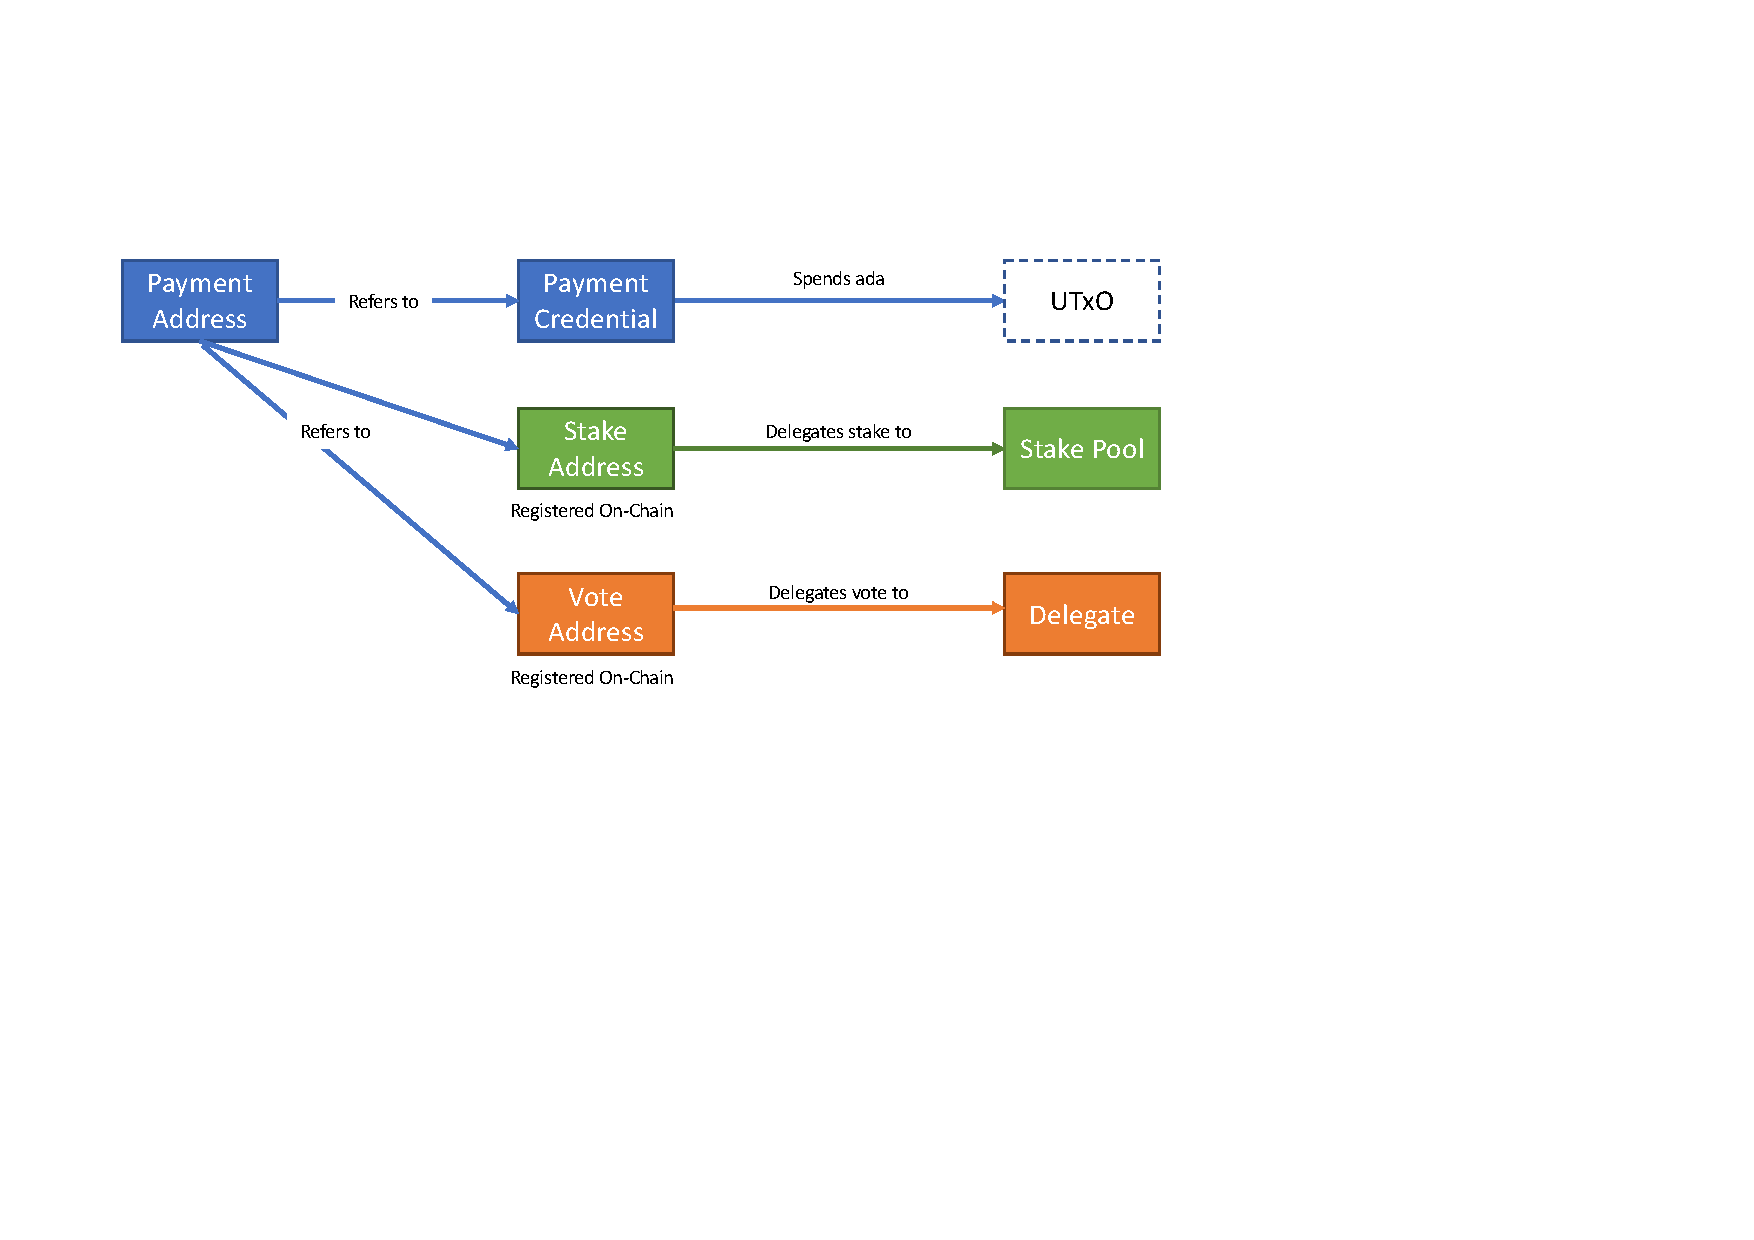
\includegraphics[trim=0 250 150 80,clip,width=\textwidth]{Indirection}
  \end{center}
  \caption{Relationship between payment addresses, payment credentials, vote addresses and stake addresses}
  \label{fig:indirection}
\end{figure*}

\subsubsection*{Payment, Stake and Vote Rights}

Figure~\ref{fig:indirection} outlines how payment addresses relate to payment credentials, stake addresses  and vote addresses.  Payment credentials are used to
authorise payments of any kind, including transacion fees.  Unspent ada is accumulated in UTxOs (Unspent Transaction Outputs).  These UTxOs may either be associated
with the payment address (so returning unspent ada to the user's account), or may be associated with some other address (so allowing ada to be transferred to other wallets,
including those owned by third parties.  If payment credentials are given to a third party, they will have full spending rights over the associated ada.  These rights cannot be
revoked without withdrawing all the associated ada. \khcomment{Not completely clear how the payment address is then removed - there's no on-chain registration.  Does it just become
useless and a target for GC?}
In Shelley, stake addresses are used to delegate block production rights.  They must be registered on chain before use.  They may be passed with the associated secret key to third parties
in order to allow them to delegate on behalf of the ada holder.  This may be useful to protect the original capital while allowing custodial delegation, for example.  Similarly,
the payment credentials may be protected by a hardware wallet, while the stake rights may be protected by software.  This may be more convenient where the hardware wallet is
held securely, for example.
In Voltaire, vote delegation is designed analogously to stake delegation.  It follows that vote rights may be passed on to the same or a different third party (or even retained), as required by the user,
and that voting rights may be asserted without needing the secret payment key.  Both stake and vote addresses may be independently de-registered at any time, in which case the associated delegation rights are immediately
revoked.  New addresses may then be created and assigned as required, and new delegations may be made.  This mechanism also provides protection against lost or stolen stake or vote keys.

\begin{figure*}[h]
  \begin{center}
  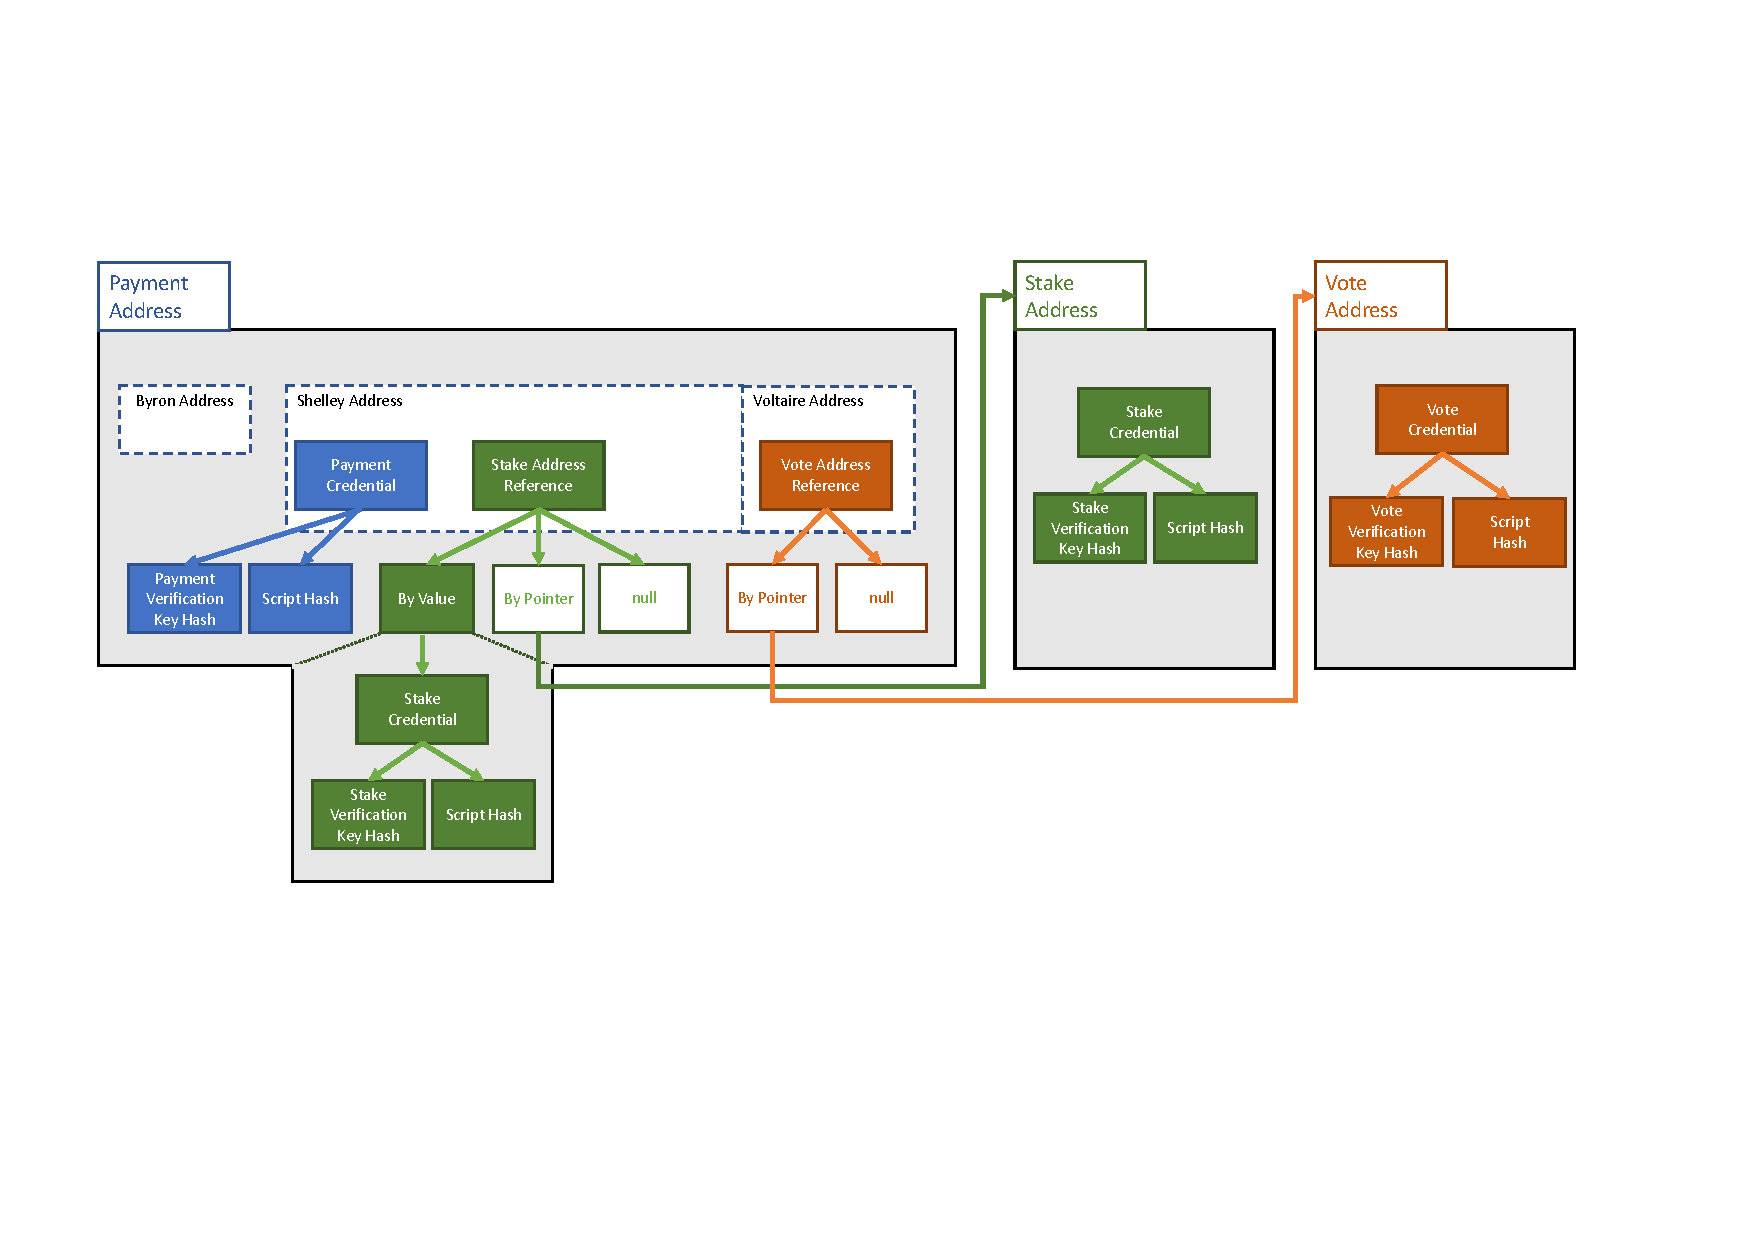
\includegraphics[trim=10 150 30 80,clip,width=\textwidth]{Address-Structure}
  \end{center}
  \caption{Payment Stake and Vote Address Structure}
  \label{fig:address-structure}
\end{figure*}

\subsubsection*{Revised Payment Address Structure}

The revised structure for payment addresses is shown in Figure~\ref{fig:address-structure} (this is adapted from the Shelley delegation design document~\cite{delegation-design}).
Payment addresses may be either Byron Addresses, Shelley Addresses or Voltaire Addresses.
\khcomment{There's apparently no on-chain registration for payment addresses.}
Voltaire addresses extend Shelley addresses by including a vote address reference in addition to the existing payment credential and stake address
reference fields.  Payment credentials may be either payment verification key hashes or script hashes.  Stake address references may be either
by value (in which case the stake credential is directly embedded in the address), by pointer to the registration transaction, or null (an efficient
form used where payment addresses do not need stake delegation rights).
Stake addresses refer to a stake credential that must either be a stake verification key hash or a script hash.
\khcomment{The Shelley address design looks over-complicated -- stake references could probably be collapsed to just pointers.}
Voltaire extends the Shelley address format by including vote address references.  These must be either by pointer to the registration transaction, or null (an efficient
form used where payment addresses do not need vote delegation rights).
\khcomment{I think the null form might not be used?  In which case we could avoid problems by eliminating it.  However, the vote address would then need either to be optional
or it would be necessary to always register the vote credentials with the payment address.}
Vote addresses refer to a vote credential that is must be a vote verification key hash.
\khcomment{The different levels seem a bit confusing.  An address is presumably a reference to the structure.  But embedded stake credentials won't have an address.  Credentials similarly
seem to always collapse down to the underlying structure (so may be naming artefects that do not really need to exist).}
\khcomment{Should script hashes be allowed as voting credentials?  I would imagine so.}
The same registration/de-registration concerns apply when pointers are used for vote address references as for stake address references (see ~\cite{delegation-design}).
Although these can be specified separately, enterprise addresses are expected to have both null stake address references and null vote address references.
\khcomment{A single null would do here for both kinds of address reference in an enterprise address, but that would be a bit harder to fit with the existing structure.}

\begin{figure*}[h]
  \begin{center}
  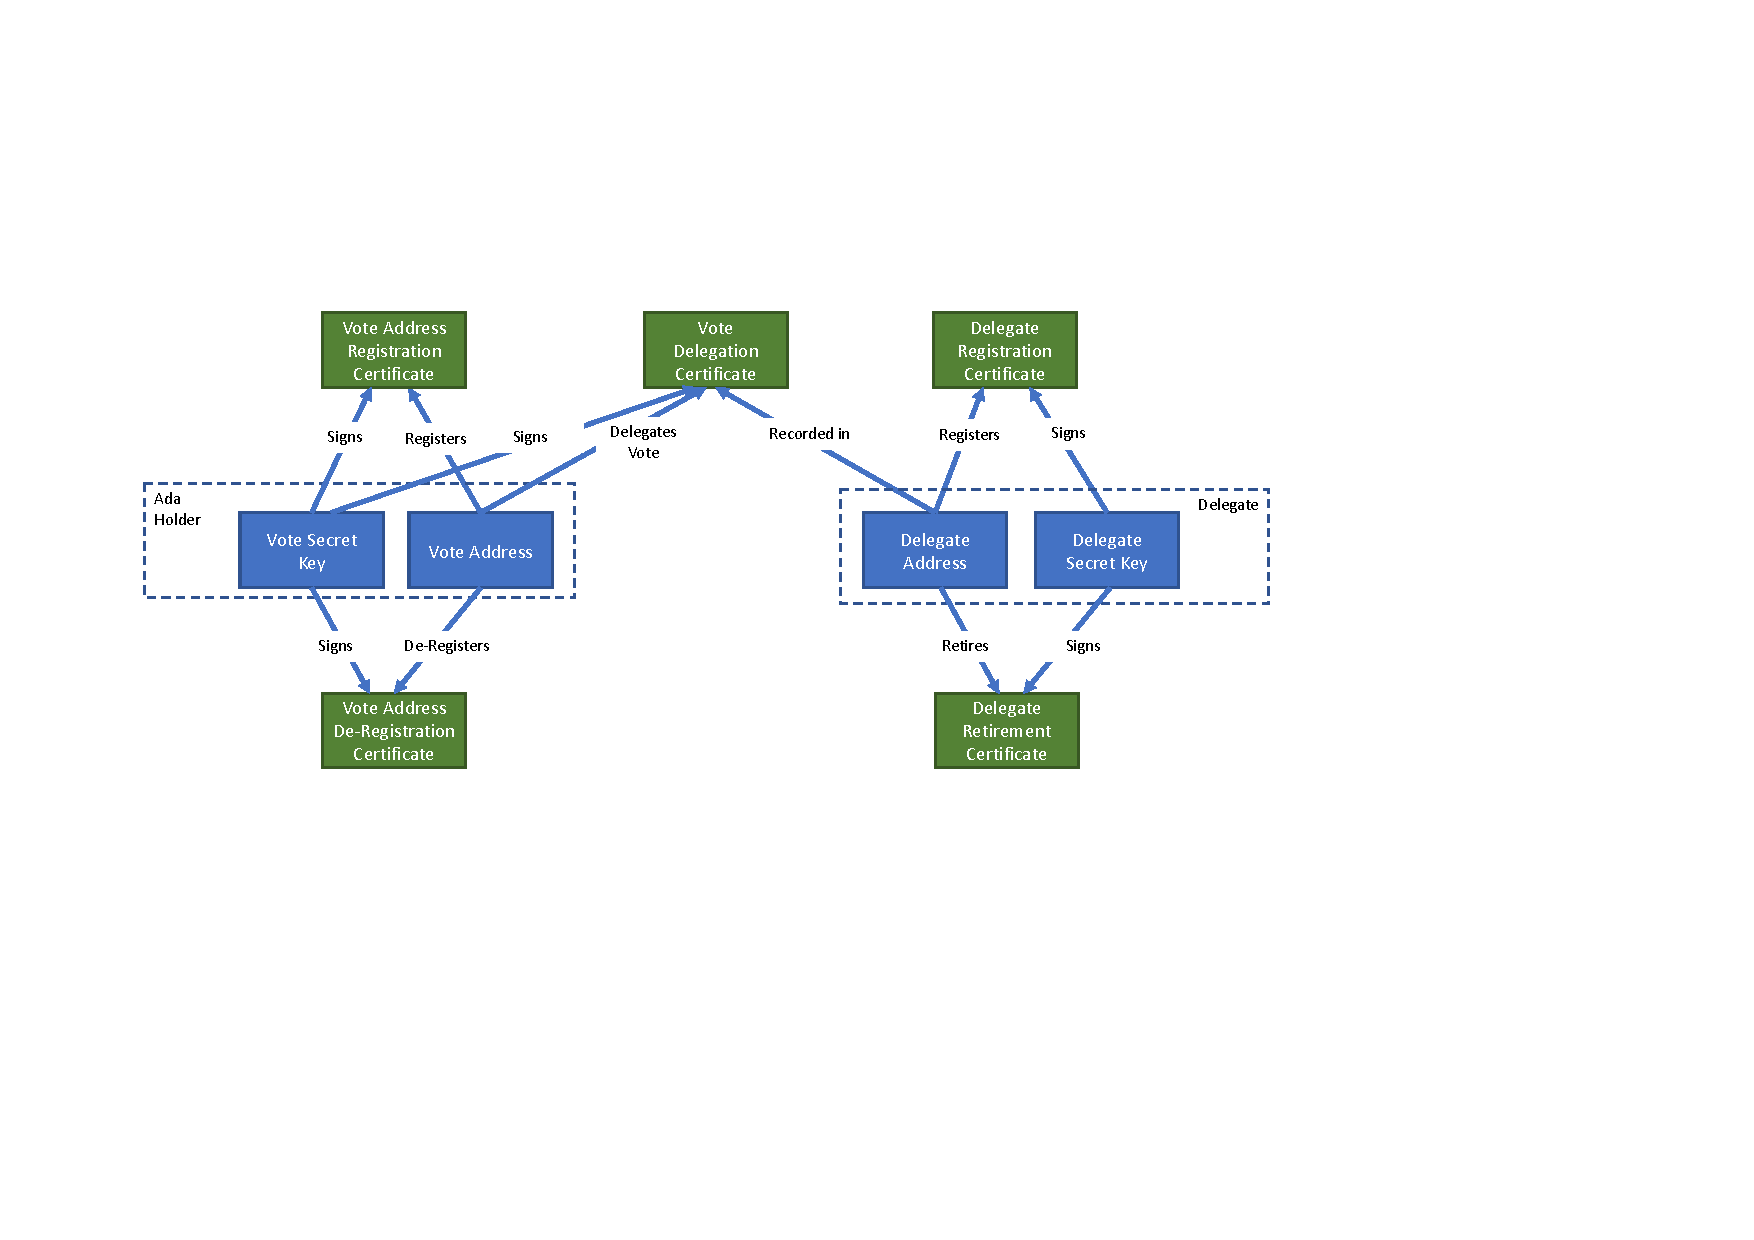
\includegraphics[trim=10 150 30 80,clip,width=\textwidth]{Relationships}
  \end{center}
  \caption{Relationships between vote addresses, keys and certificates}
  \label{fig:relationships}
\end{figure*}

\subsubsection*{Certificates and Registrations}

The Shelley design supports the following kinds of registration certificate to cover the registration/de-registration of stake addresses and stake pools on the blockchain:

\begin{itemize}
\item
Stake address registration certificate;
\item
Stake address de-registration certificate;
\item
Stake delegation certificate;
\item
Stake pool registration certificate;
\item
Stake pool retirement certificate;
\item
Stake pool operational key certificate.
\end{itemize}

The Voltaire design adds the following in an analogous way:

\begin{itemize}
\item
Vote address registration certificate;
\item
Vote address de-registration certificate;
\item
Vote delegation certificate;
\item
Delegate registration certificate;
\item
Delegate retirement certificate;
\end{itemize}



The relationships between these certificates and the vote address and vote keys is shown in Figure~\ref{fig:relationships}.
This is analogous to the design for stake addresses and certificates.
\khcomment{The actual relationships between keys, addresses and certificates are rather unclear in the stake delegation design document.  I think this is correct
but the original document might need to be fixed up...
It's not quite clear when things should be public keys and when they need to be addresses, or which things need actually to be included in the certificates.}
However, unlike the Shelley stake delegation design, the vote design does not need a cold/hot (KES) key structure, a VRF key, or an operational certificate.
\khcomment{I assume hot/cold isn't needed, since security is not directly affected, but I may be wrong?  VRF and operational certificates are certainly not needed.}

\subsubsection*{Certificate Precedence and Validity}

The blockchain specifies a strong and verifiabe temporal ordering on events.
Newer vote, vote delegation, and delegate certificates always override older ones.  Certificates remain in force until they are revoked or a newer certificate is issued,
whichever comes first.  Vote and delegate certificates may be revoked.  Vote delegations are not explicitly revoked, but are only valid when both the vote certificate
and delegate certificate are also in force.
Newer delegation certificates override older delegation certificates. This allows delegators to move from one stake pool to another.

\newpage
\section{Voting on Proposals (On-Chain, Delegates)}
\label{sect:voting}

Once a properly signed proposal has been submitted on-chain, delegates may vote on whether or not to accept it.  A threshold is set for each vote.
As described in Section~\ref{sect:submission}, the thresholds for each proposal are included in the formal proposal at submission time.

\subsection{Voting}

Each \emph{registered} delegate (see Section~\ref{sect:registration}) may vote either in favour or against a proposal by submitting the corresponding transaction.  They may change their vote up to the point
where the vote is tallied.  Any changes after that point in time are not considered.  If a delegate chooses not to vote on a proposal, that is considered to be
a vote against the proposal.  Votes are submitted in the form of an on-chain transaction, and may incur fees.  The transaction needs to include:

\begin{center}
\begin{tabular}{||l|p{3in}|l||}
  \hline\hline
  proposal id & The unique identifier for the proposal, derived from the submission & 32 bytes
  \\\hline
  vote intention & Yes or no & 1 byte
  \\\hline
  Delegate public key hash & Unique identifier & 32 bytes
  \\\hline
  \hline
\end{tabular}
\end{center}

This ensures that there is a public and traceable record of each delegate's actual vote.


\subsection{Stake Snapshots}

Stake snapshots are taken at the start of each epoch.  These snapshots are currently used only for block production purposes, but they will be reused here for governance purposes.
The stake snapshot that is taken at the start of an epoch will be used for all delegated votes that are tallied at the end of the epoch.
The same stake snapshot that is used for block production is also used for endorsement.
As with block production, using fixed snapshots means that there will be a
slight delay before a change in stake will be effective for voting purposes.
However, this brings major efficiency advantages (it is not necessary to calculate specific snapshots per vote).

\begin{figure}
  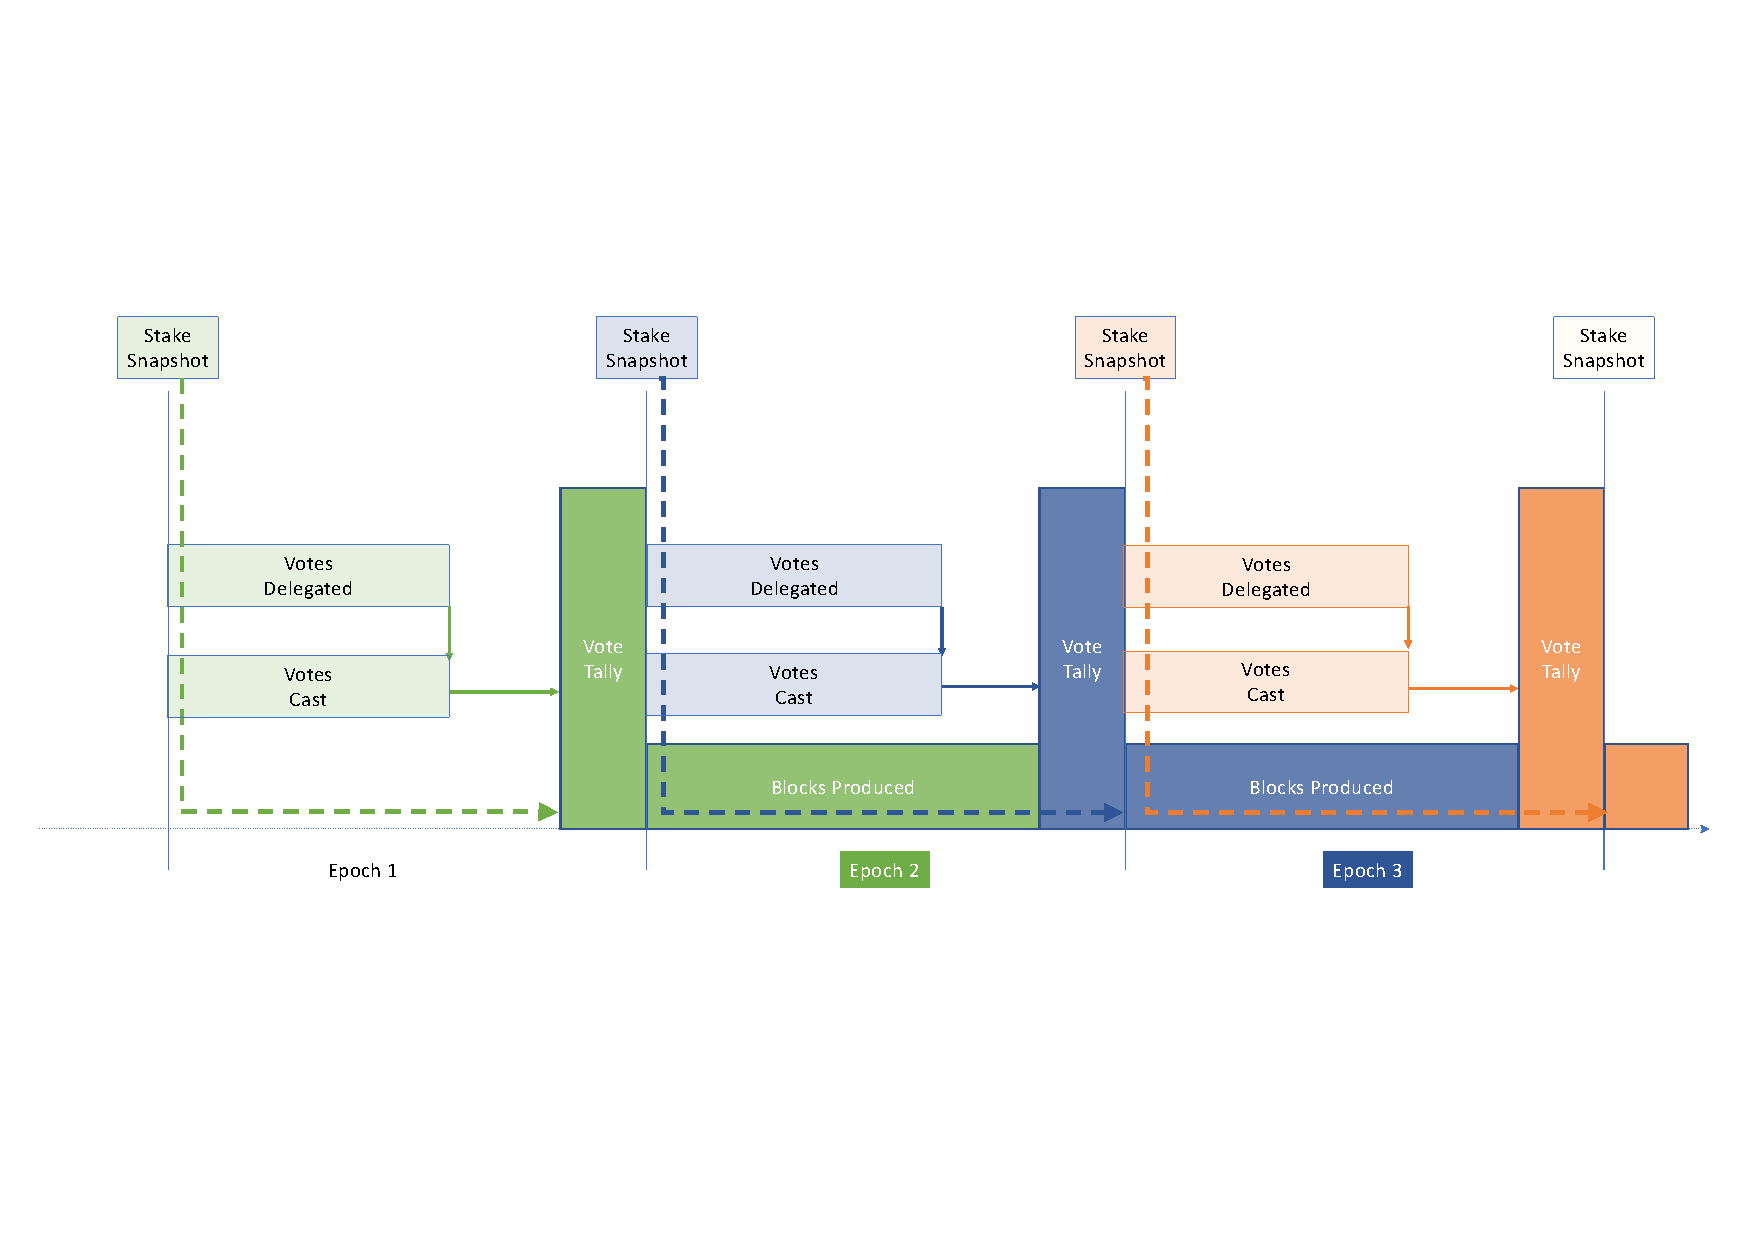
\includegraphics[trim=0 150 0 80,clip,width=\textwidth]{Stake-Snapshots}
  \caption{Stake Snapshots}
  \label{fig:stake-snapshots}
\end{figure}

Note that because of the lag in block production delegation, this design means that vote and block production stake will not be exactly aligned in an epoch.
%\khcomment{It seems sensible to separate the vote and block production snapshots like this, but it does give a slightly odd effect, in that vote and block production stake
%  will not always be the same in a given epoch.  They could be aligned, but then there will be a lag in the vote.}

 

\subsection{Tallying Votes}

Votes are tailied according to a snapshot of delegated vote that is taken at the specific point given in the proposal submission.  The stake snapshot from the start of the epoch is used to determine
the weight of each delegated vote for all votes that are tallied at the end of the epoch.  The total vote that is controlled by each delegate is the sum of all active delegations at the point that
the vote is tallied.  A calculation is made for the total amount of stake that is: i) explicitly in favour and; ii) explicitly against the proposal.  This is compared against the required voting thresholds and
if sufficient votes have been achieved, then the proposal will be accepted as decscibed below.
The tally needs to be recorded on chain.
%\khcomment{Does the tally need to be recorded on chain?}

\subsection{Voting Outcomes and Thresholds}

Following the tally, a proposal may be either accepted or rejected, based on whether it has achieved the required voting threshold.  Any proposal that achieves at least
the specified percentage of votes is accepted, and passed forward for future enactment.
The threshold for accepting a specific vote is specified in the proposal.
This must be no less than any relevant minima that are set in the protocol parameters for the specific type of proposal.
% \khcomment{there may also be minima that are set in the protocol parameters.}.
All thresholds are specified as a percentage of total ada.  There are a number of ways that this total can be specified.  In roughly declining order of size, these include:

\begin{enumerate}
\item
  The total ada that is in existence (i.e. 45 billion ada).
\item
  The total ada that is in circulation (i.e. that is not accounted in either the treasury or reserves pots) (Preferred).
\item
  The total ada that has been delegated for block production purposes in the current epoch (Preferred).
\item
  The total ada that has been delegated for voting purposes in the current epoch.
\item
  The total ada that has been used to cast a vote on a specific proposal.
\end{enumerate}


A decision needs to be taken on how to determine the total that is used in a threshold calculation\footnote{It makes sense to use the same total for all votes rather than using different totals
  for different kinds of vote.}.
Using the total ada in existence (option 1) means that very high voting thresholds cannot be achieved until all ada
is in circulation, and that ada that has not been circulated will always have a negative effect on voting.
This seems undesirable.
The second option avoids this issue, but means that ``inactive'' ada will count as a vote against a proposal, which may prevent the chain from making reasonable progress.
The third option ensures that all ``active'' participants in the blockchain are considered, but could in theory give results greater than 100\% (because of lag in the
block production snapshot compared with the voting snapshot, or if vote delegation is more popular than block production delegation).
While the fourth option may seem attractive, it may result in highly unrepresentative results if insufficient stake holders choose to delegate their vote.  This would potentially allow control of the
blockchain to be circumvented at low attack cost, so creating a security vulnerability, and would also create potential instability in the blockchain.
Likewise, the fifth option would allow proposals to pass with very little positive mandate (e.g. where only 10\% of the delegate group chose to vote on a specific issue, a majority vote could be
achieved with just over 5\% of the delegated stake).
The Priviledge project has developed further metrics that could be used to set the thresholds based on e.g. the proposal type and the
impact on the system.

\subsubsection*{Low Thresholds and Explicit Negative Voting}

One option is to require both positive and negative thresholds for a vote.  This might allow lower voting thresholds.
This approach has a number of disadvantages, however:

\begin{itemize}
\item
  The thresholds could not, anyway, be lowered significantly (or perhaps at all) without permitting unrepresentative outcomes in terms of
  favourable stake -- lower thresholds could only be accepted for certain kinds of proposal -- setting thresholds below 50\% would be hazardous, for example;
\item
  Delegates who control other delegation are already socially motivated to vote.  Delegators will remove their delegation from delegates who consistently fail to vote,
  and may require explanations for any proposal where no vote is given.
\item
  It imposes a per-vote transaction cost on normal ada holders who have chosen to register as their own delegates, and this may not be sustainable for small holders.
  This then works to reduce the number of ada holders who choose to register as delegates, consequently increasing centralisation\footnote{This assumes there is no compensation or incentive to encourage voting.}
  (Conversely, normal ada holders who do register as delegates must be positively in favour of/against a proposal by paying the requisite fee -- this acts as a deliberate drag
  to ensure some conservativism/stability in the system).
\item
  It adds complication and opportunities for gaming (eg with careful setting of thresholds);
\item
  Votes are registered on chain.  It may be socially unacceptable for a normal ada holder to vote explicitly against a proposal.  This allows an individual to have a ``silent'' negative vote.
\item
  Care needs to be taken over increasing execution costs. Tallies are potentially a critical point of performance failure, and this could perhaps double
  the cost for each tally.  High tally costs could even mean that some proposals were rejected (if they were not completed by the required deadlines, for example).
\end{itemize}

\newpage
\section{Endorsement of Proposals (Endorsers, Needed only for Protocol Version Changes)}
\label{sect:endorsement}

Proposals that change either or both the major or minor protocol version number (``hard forks'') need confirmation from the block producing nodes that they are able
to deal with the new protocol.  We term this ``endorsement''.   In previous Cardano eras, endorsement has been handled manually, as a judgement call that
is made by the blockchain operators, who are in control of the genesis keys and the core block producing nodes.  As we move away from federated control and eliminate these
mechanisms, it is necessary to automate this process.  Major protocol versions will never decrease.  Minor protocol versions will always either increase or be set to zero
(with a corresponding increase in the major protocol version number).

subsection{Automating Endorsement}

Every block producing node (``stake pool'') that wishes either to continue minting
blocks or to support the distributed verification of the Cardano blockchain must upgrade its
software to a node version that is compatible with the new protocol.  So that it
can follow the blockchain from its inception (that is, from the genesis block),
the new node software must also be prepared to handle any previous version of
the protocol, that is from version 1.0 (Byron) through all intermediate versions to the current protocol version.

There are several obvious ways that could enable an \emph{endorser} to endorse a protocol version upgrade.  A decision needs
to be made on which of these to use.

\begin{description}
\item
  [Manual endorsement.]  The endorser submits a signed transaction on-chain that confirms the maximum protocol version that they are
  able to accept (or submits an endorsement transaction for a specific proposal id).
\item
  [Automatic endorsement.]  The new software submits a signed transaction on-chain that confirms the maximum protocol version that it is
  able to accept.
\item
  [Automatic endorsement by statistical count of blocks produced.]  Each block includes the protocol version that is used by the pool that minted it.  This can be used to
  estimate the percentage of stake that is controlled by upgraded pools.
\item
  [Automatic endorsement by stake.]  Each block includes the protocol version that is used by the pool that minted it.  A map is used
  to record the most recent protocol version that is being used by each pool.  The total stake that is controlled by upgraded pools can then
  be calculated at the time of endorsement using the stake snapshot.
\end{description}

% In  cases, the transaction will need to be signed by the stake pool operational key.
Automatic endorsement has the advantage that it will always record the current
status of the pools (including any downgrades).
% However, it is not obvious that a specific proposal (identified by the proposal id) could be endorsed
% automatically.
Manual endorsement allows endorsers to have better control over
the timing of their endorsement (for example, when testing a new node version)
and to endorse specific proposals rather than a protocol version (so avoiding issues if two proposals
mistakenly refer to the same protocol version).  However, some
endorsements may be missed, and consequently some upgrade proposals might not be enacted
even though nodes are actually able to handle the new protocol.
Automating endorsements by block production reduces the number of transactions that are needed (and so reduces overhead costs for pool operators),
but unless the stake snapshot is used, this will only give a statistical measure of the upgrade status (some percentage of blocks have been produced by
pools that have upgraded).
% It may be necessary to restrict the period of endorsement to the time between proposal submission and vote tallying.
% \khcomment{Are there situations where it might make sense to upgrade pre-emptively before a proposal is submitted?}

\subsection{Tallying the Endorsements}

Endorsements are tallied following the deadline that is given in the proposal.
If there is sufficient endorsement for the proposal, then it will be carried
forward for enactment.  While the endorsement deadline is technically
independent of the voting deadline, in practice it will usually be later than the
voting deadline. That is, first the vote will be taken, then pools will indicate
their readiness to proceed with the protocol version upgrade, and if both thresholds are met,
then the proposal will be enacted.

The endorsement threshold is separate from the voting threshold, and also
may be set per-proposal.  % If the endorsement threshold is met, then the proposal is passed for enactment.
In contrast to voting, the total amount of stake that has been delegated for block production purposes is used to determine this
threshold. % \khcomment{I think it makes sense to
%   use the same snapshot that is used for normal block production rather than the
%  most recent delegation snapshot, but this should be discussed.}
To avoid chain forks, the minimum threshold for endorsement must not be less than 50\%
of the block producing stake, but may need to be higher to account for statistical variation or any errors etc.
If statistical block production is used, then the threshold should be set as a percentage of the blocks that have been produced.
This threshold should be set conservatively (e.g. a minimum of 60\% of the blocks produced).

\newpage
\section{Proposal Enactment}
\label{sect:enactment}

When the stated deadline for a proposal is reached, then it is considered for enactment.  Proposals are never considered for enactment
before the deadline.  A proposal that has been accepted by passing a voting threshold (and also, for a protocol version upgrade, the
endorsement threshold) is automatically enacted.  Enactment involves each protocol parameter being updated to the new value that is specified
in the proposal.  Changes take effect at the start of the following epoch.  A protocol version upgrade can also update other parameters as part of
the proposal, and may even change the set of parameters that can be updated.

\subsection{Protocol version changes (``Hard Forks'')}

Protocol version upgrades never decrement the protocol version.  They must increment either the current major or the current minor version by one.
If the major version is incremented, then the minor version must be set to zero.
% may be set to any required value (usually this will be zero).
Software upgrades must accept all prior protocol versions (both major and minor) that have been successfully enacted.
When a protocol version proposal is enacted, then all nodes will synchronise to the new protocol version using the ``hard fork combinator''~\cite{hardfork-combinator}.
Block production and verification will continue at the start of the next epoch using the rules that are in force for the new protocol version.

\paragraph{Major version changes override minor version changes.}
Under these rules, the only possible conflict is where one or more properly approved and endorsed proposal increments the major version and another increments the
minor version in the same epoch.  In this case, the major version change will always succeed, regardless of the order in which the proposals are enacted: if the major version change is enacted first,
then any subsequent minor version change will be invalidated.  Conversely if the minor version upgrade is enacted first, then it will be overridden by the subsequent major version upgrade.

\subsection{Prioritisation of Enactment}

If multiple update proposals are to enacted within a single epoch, then they are enacted strictly in the order that they were submitted.
This creates a deterministic order that does not need to consider when proposals achieve a majority vote, for example.
It allows proposals to be completely or partially overridden without needing an explicit cancellation option.
This approach assumes, of course, that the submitter group acts honestly and in the best interest of the protocol.
The approach does not allow contingent/conditionals proposals.  If needed, this can be handled by, for example, submitting two separate proposals that are enacted
in different epochs, where the second proposal is submitted only if the first proposal succeeds.

\subsection{Central Funds Transfers (``MIRs'')}

Several proposals for funds transfers may be enacted in a single epoch.  These proposals are enacted the in the order that they were submitted, with all ledger and
accounting rules in force.  In particular, it is not possible for the treasury, reserves or any private address to even temporarily have a negative balance.  This may affect
the ordering of transfers in some edge cases.

\section{Deadlines and Stability Windows}

% \subsection{Deadlines}

% \subsection{Timing and Stability Windows}

In order to ensure the stability and security of the blockchain, it is essential that updates are known sufficiently in advance of an epoch boundary.
Independent deadlines may be set for voting and endorsement.  These deadlines must respect these timing and stability constraints.
The constraints are as follows.

\begin{tabular}{||l|p{2in}|p{3in}||}
  \hline\hline
  \textbf{What} & \textbf{When} & \textbf{Description} \\
  \hline
  Submission & Within 2 stability windows of the start of an epoch & \\
  \hline
  Voting & No less than 1 stability window before the end of the epoch prior to enactment & \\
  \hline
  Endorsement & No less than 1 stability window before the end of the epoch prior to enactment & \\
  \hline
  Enactment & At a specific epoch boundary & \\
  \hline
\end{tabular}

\section{Rewards Mechanism (On-Chain and Off-Chain)}

No on-chain rewards are currently envisioned for either voters or delegates.   Rewards may be offered for participating in the off-chain voting process.


\clearpage
\addcontentsline{toc}{section}{References}
\bibliographystyle{plainnat}
\bibliography{references}

\todo{Add in any necessary references.}

\appendix

\clearpage
\section{New Protocol Parameters}
\label{sec:parameters}

\begin{tabular}{||p{2in}|p{2.8in}|p{0.5in}|p{0.4in}||}
  \hline\hline
  \textbf{Parameter} & \textbf{Description} & \textbf{Initial Setting} & \textbf{Updat\-able}
  \\\hline
  \texttt{MinVote} & Minimum Allowable Threshold for Voting & 50\% & Y
  \\\hline
  \texttt{MinEndorse} & Minimum Allowable Threshold for Endorsement & 75\% & Y
  \\\hline
  \texttt{MaxEnact} & How far in Advance of Enactment can a Proposal be Submitted & 3 epochs & Y
  \\\hline
  \texttt{ProposalQuorum} & What is the Minimum Number of Signatories that is Required on a Proposal & ? & Y
  \\\hline
  \texttt{MaxDelegateRetire} & How far in Advance can a Delegate Announce their Retirement & 5 epochs & Y
  \\\hline
  \texttt{MinDelegateRetire} & How far in Advance must a Delegate Announce their Retirement & 0 epochs & N
  \\\hline
  \texttt{LatestEndorsementDeadline} & By Which Slot in an Epoch must a Proposal be Endorsed if it is to be Enacted & ? & N
  \\\hline
  \texttt{LatestVotingDeadline} & By Which Slot in an Epoch must a Proposal be Voted on if it is to be Enacted & ? & N
  \\\hline
  \hline
\end{tabular}

The \texttt{ProposalQuorum} setting will need to be a sensible proportion of the submitter group. Note that \texttt{MinDelegateRetire} may be built in to the protocol rather than a parameter.


\section{New Genesis File Settings}
\label{sec:genesis}

Some additions need to be made to the genesis file.


\begin{tabular}{||p{1in}|p{4.7in}||}
  \hline\hline
  \textbf{Setting} & \textbf{Description}
  \\\hline
  \texttt{submitters} & List of hashes of public keys for the submitter group
  \\\hline
  \hline
\end{tabular}

The \texttt{submitters} entry gives a list of public keys for the initial submitter set.  This can be modified by registering additional submitters.


\clearpage
\pagebreak
\section{Efficiency Concerns}
\label{sect:efficiency}

This appendix considers possible efficiency concerns.  Overall, the design will lead to some (limited) increase in memory
usage (proportional to the number of registered vote addresses), plus some additional transaction costs.
Proposal submission and enactment should carry minimal additional costs compared with the current manual process.
Additional costs are associated with vote snapshots, registration, vote delegation, and vote tallying.
These costs are bounded by the product of the number of vote delegations and the number of active proposals.
Overall, the costs are manageable and proportionate, provided that there are not a large number of active proposals.
It may be advisable, however, to group a set of proposals under a single vote.

\subsection{Proposals and Proposal Submission}

A single proposal needs to be submitted with appropriate signatures.  The cost of this submission should be no greater than
a normal transaction submission.  Proposals need to be stored for voting and enactment.  An in-memory hash is sufficient
for each proposal up to the point of enactment.  This hash could be recorded on-chain.

Assuming that the majority of the submitter group is honest, then the number of proposals that are under consideration
at any point in time should be small and finite.  By setting time limits on enactment, this number can be controlled.

Since there is likely to be at most only one or two active protocol upgrade proposals, and a small number of active parameter
changes, the most significant pressure is likely to come from funds transfer proposals (``MIRs'').  Because only a relatively
small number of transfers can be included in a single proposal\footnote{Around 100-200}\todo{check this number},
a single high-level funding decision could, in principle, result in several on-chain proposals.
Submitters should take care over the number of such proposals, and consider submitting them over multiple epochs, if possible.
If this is expected to be common, then it may be sensible for a single vote to activate a group of proposals.
This will reduce the number of vote transactions, as well as reducing the risk of voter fatigue (or only part of a group
being authorised).


% It is necessary to avoid ``flooding'', where many junk proposals are subm.

\subsection{Vote Snapshots}

It is necessary to take vote snapshots before tallying votes.  Since different
credentials are used for vote and stake delegation, this is in addition to the
usual stake snapshot.  Unlike stake delegation, only a single active snapshot is required.
It is not necessary to calculate this during the epoch transition, provided that it is available
at the point at which any votes are tallied.  It follows that the snapshot could be calculated
incrementally, if desired.  This would reduce calculation pressure.  There are approximately 420,000
registered stake addresses\footnote{2021-04-09}.  Storing a similar number of vote addresses would require approx. 15MB of
memory\khcomment{assuming 28 bytes for an address hash, 4 bytes for a value, and 4 bytes for a header word.}.

\subsection{Vote Delegation}

A one-off cost (time/ada/chain growth) is paid for registering each vote delegation
key.  This will be similar to the cost that is paid for e.g. registering a stake key.
At most one key must be registered for each active payment credential.
Certificates are registered on-chain.  There is no direct impact on the size of
the UTxO.  A similar cost is paid each time a vote delegation is made or changed.

\subsection{Delegates and Voting}

A one-off cost (time/ada/chain growth) is paid for registering each delegate.
This will be similar to the cost that is paid for e.g. registering a stake key.
Delegates must also submit votes.  There will be one vote transaction per delegate per proposal.
Assuming that there is a small number of active proposals and the number of delegates is
significantly less than the number of registered voters, we can estimate the typical number of
votes per epoch to be less than 10,000. This would be covered by around 500s of total transaction time.

\subsection{Vote Tallying}

Tallying the vote involves summing the delegations that have been made in favour of each active proposal.  Since delegation can be
changed up to the point where a tally is taken, this must be done after the tally point and prior to enactment.
In the worst case, each tally involves adding the stake that is associated each delegated vote (potentially \emph{420,000}
additions).  This can, in principle, be parallelised and provided that sufficient time is available between the tally
and the proposal enactment, can be carried out incrementally.  Limiting the number of active proposals will also
limit the total computational time.
The total possible delegation can be pre-calculated from the snapshot, so should not add significantly to performance costs.

\subsection{Endorsement}

Automatic endorsement carries minimal time overhead.  As each block is produced, the corresponding  pool identifier needs to be
recorded.  The total stake that is prepared to upgrade needs to be calculated prior to the endorsement.  Assuming that there are
approximately \emph{2k} block producing pools and \emph{k} is 2,500 or less, this will involve a maximum of 2,500 additions,
which should have negligible performance impact.

\subsection{Enactment}

Automatic endorsement carries minimal time overhead.  As each block is produced, the corresponding  pool identifier needs to be
recorded.  The total stake that is prepared to upgrade needs to be calculated prior to the endorsement.  Assuming that there are
approximately \emph{2k} block producing pools and \emph{k} is 2,500 or less, this will involve a maximum of 2,500 additions,
which should have negligible performance impact.

\subsection{Voting Centre}


\clearpage
\section{Off-Chain Process}
\label{sect:off-chain}

This appendix outlines possible off-chain processes, and how they would interact with the on-chain process that is the focus of this design document.

\subsection{Voter Registration}

The Catalyst system requires voters to register prior to casting their votes.  This is not needed for the on-chain process, since it is possible to take a
stake snapshot directly for each voting address. Votes may then be delegated simply by issuing an on-chain transaction, without requiring any explicit registration.
% \khcomment{There seems to be no good reason to exclude ada holders from on-chain voting simply because they have not registered for off-chain Catalyst voting?}
As discussed in Section~\ref{sect:rewards}, rewards are only issued to those who do register for off-chain voting, so there is already an incentive to participate
in the voting process.

\subsection{Proposal Implementation}

On-chain proposals must follow the precise format that is given in Section~\ref{sect:submission}.

\paragraph{Proposal Editors.}  May be involved to confirm that the proposal is documented according to the required procedures, and that the change is properly recorded.

\paragraph{Technical Experts.}  May be involved to formulate the proposal and ensure that it is processed according to the procedures.

\paragraph{Software Developers.} Will be involved to implement new node and other software that is required by a new protocol version.

\paragraph{Security Experts.} Will be involved to advise on the effects of parameter changes, and to advise on the security implications of new software.

It is important that all deadlines are specified precisely in any on-chain proposal, and that sensible deadlines are chosen, based on the type of proposal and any
voting decision that has been made.  It is also essential that all requirements are followed in terms of submission times, stability windows signing etc, so that a proposal is not
rejected unnecessarily.


\subsection{Relating on-chain and off-chain proposals}
\label{sect:relating-off-and-on-chain}

It may be necessary to relate off-chain discussion and decisions to the corresponding on-chain proposal and enactment.  The unique proposal
identifier allows a proposal to be tracked on-chain, but does not link it directly to off-chain discussion.

\begin{description}
\item [Manual.]
  A member of the community (eg the proposal submitter), creates the link.  The proposal is tracked automatically through an on-chain explorer, and the result is
  displayed in a form where it can be tracked by the original voting group or other interested parties.
\item [Automatic.]
  An identifier is constructed following a successful off-chain vote.  This could be a hash or some other form.  The identifier is used by the proposal implementors and editors, and is embedded
  in the proposal implementation.  The identifier is linked to the on-chain identifier, and the progress of the proposal is then tracked automatically on-chain, as described above.
\end{description}

In both cases, it may be possible or even necessary for multiple on-chain proposals to refer to the same off-chain identifier.  This could happen where, for example:

\begin{itemize}
\item
  An incorrect proposal is submitted on-chain.
\item
  A proposal fails to be enacted for some reason, and a new version is therefore submitted on-chain.
\item
  An off-chain proposal gives rise to multiple on-chain proposals.  For example, multiple independent funds transfers might be submitted as the result of a single
  decision; independent proposals might be submitted for each of two parameter changes; a protocol version might be upgraded and some specific parameter settings made independently;
  parameters might be changed over repeated epochs (e.g. to gradually increase/decrease some parameter); parameters might be changed in one epoch, in preparation for a protocol version
  change in a subsequent epoch.
\end{itemize}

Tracking proposals in this way helps preserve continuity, and provides explanations for enacting specific on-chain proposals.  This will be especially helpful where many proposals
are simultaneously under consideratation.


\subsection{Security Threats.}

In most cases, security threats should not be made public until a fix has been prepared, and ideally until it has been enacted on-chain.  This mitigates the risk of
security vulnerabilities affecting the continuity of the blockchain. However, it creates a conflict with the
principle of full decentralisation and transparency of government.  An acceptable process needs to be developed that will meet the required security and openness goals.
\emph{In particular, it may be necessary to prioritise security over transparency, and to accept lower levels of decentralisation.  It may also be necessary to consider
  the legal implications of specific actions or governance structures.}
While vulnerabilities in the node or other software may be fixed out-of-band, without needing any governance mechanism,
security vulnerabilities in the protocol will, of course, usually require a protocol version change (``hard fork'').

\TODO{Survey the literature on blockchain security and open governance, and consider solutions that have been proposed.  Priviledge does not directly consider security, as far as I am aware?  It allows
  proposal prioritisation and deadlines, which provide one way to help deal with security problems.}

\TODO{Take input from the IOG security group.}

Possible approaches include:

\begin{itemize}
\item
  Allow security issues to completely bypass the off-chain discussion, ideation and voting phases.  Appoint a committee of experts to assess security threats.
  Ensure that security threats are classified, and prioritise the implementation of solutions to those threats.  Where the protocol needs to be changed, ensure that this
  proposal has sufficient priority.  Proposals should still comply with implementation requirements, but there may be a moratorium on documentation until the proposal has
  been enacted.
\item
  Allow security issues to bypass discussion and ideation, but then follow the usual voting, implementation, checking etc process.  This may be appropriate for low threats,
  or ones that cannot be easily enacted without rapid detection and response, but raises significant risks where a major or easily exploited vulnerability has been found.
\end{itemize}


\subsection{Legal Issues}

Legal input needs to be taken on the governance structure.  In particular, care needs to be taken over group liability.  Indemnity insurance may be necessary or advisable when
undertaking some roles.

\TODO{Obtain legal input before setting up the procedures.}


\subsection{Scope of Governance Issues}

The PUP mechanism is confined to:

\begin{enumerate}
\item
  changes in updatable protocol parameters;
\item
  protocol version upgrades (``hard forks'');
\item
  central funds transfers (``MIRs'').
\end{enumerate}

Decisions that are taken on parameter and protocol version updates will generally be highly technical.  Discussion may be confined to expert groups, implementation made by
technical experts, and delegates will usually be drawn from those with significant technical expertise.  Decisions must be made in a timely manner, with on-chain enactment.
It may be necessary to establish a separate governance track, different voting thresholds, and specific procedures for such decisions, including some way to prioritise and
filter business.


\clearpage
\section{Transitioning to Decentralised Governance}
\label{sect:transition}

The move to automated decentralised governance is irreversible.  In order to mitigate security and other implementation risks, and to ensure that the off-chain and on-chain
processes are sufficiently robust, it is sensible to undertake a number of pilot studies prior to enabling full on-chain automation.

\subsection{On-Chain Pilot}

Initially, pilots can be used where governance decisions are taken off-chain, and then enacted on-chain using the existing manual update process from Shelley/Allegra/Mary/Alonzo.
As part of these pilots, some or all genesis delegate keys could initially be devolved to community members (perhaps in a time-limited way).  This immediately reduces centralisation,
but doesn't enable full autonomy or introduce additional governance checks.

A second pilot could then involve implementing a testnet that can be used to mimic the automated on-chain process.  This has the advantage of allowing the full on-chain automated
process to be tested, with governance decisions enacted on mainnet, without needing to process the hard fork on-chain.  That reduces both timing risk and any risk from failed automation.
The following steps are necessary.

\begin{itemize}
\item
  Stake snapshots must be produced that are to be used in the testnet.  Two snapshots may be needed: one for endorsement and one for voting.  The snapshot must include
  test ada for all those who should be involved in the vote.
\item
  Delegates register on the testnet.
\item
  A formal proposal is prepared and submitted to the testnet.
\item
  Ada holders delegate their vote to registered delegates.
\item
  Delegates vote on whether or not to accept the proposal.
\item
  Assuming the proposal is accepted, it is passed for endorsement (if necessary).
\item
  A proposal that is accepted and endorsed is enacted on the testnet.
\item
  Assuming it has been enacted on the testnet and there are no security or other concerns, an identical proposal is submitted on mainnet and the usual manual steps are
  followed to enact the proposal.
\end{itemize}

It is recommended that the pilot proposal be for either some specific funds transfer, or for some simple parameter update, rather than for a protocol version.

\subsection{Off-Chain Governance}

The full governance chain will also need to be tested on an end-to-end basis.  An idea will need to be discussed and a proposal submitted for formal off-chain voting.  Assuming it is not rejected,
the proposal will need to be implemented, checked for any security issues, passed to an implementor group, checked and recorded by the CIP editors, then submitted on-chain.
Depending on timings, this can be done either through the initial on-chain pilot, though the manual process, or through the on-chain automated enactment process.

\begin{figure}
  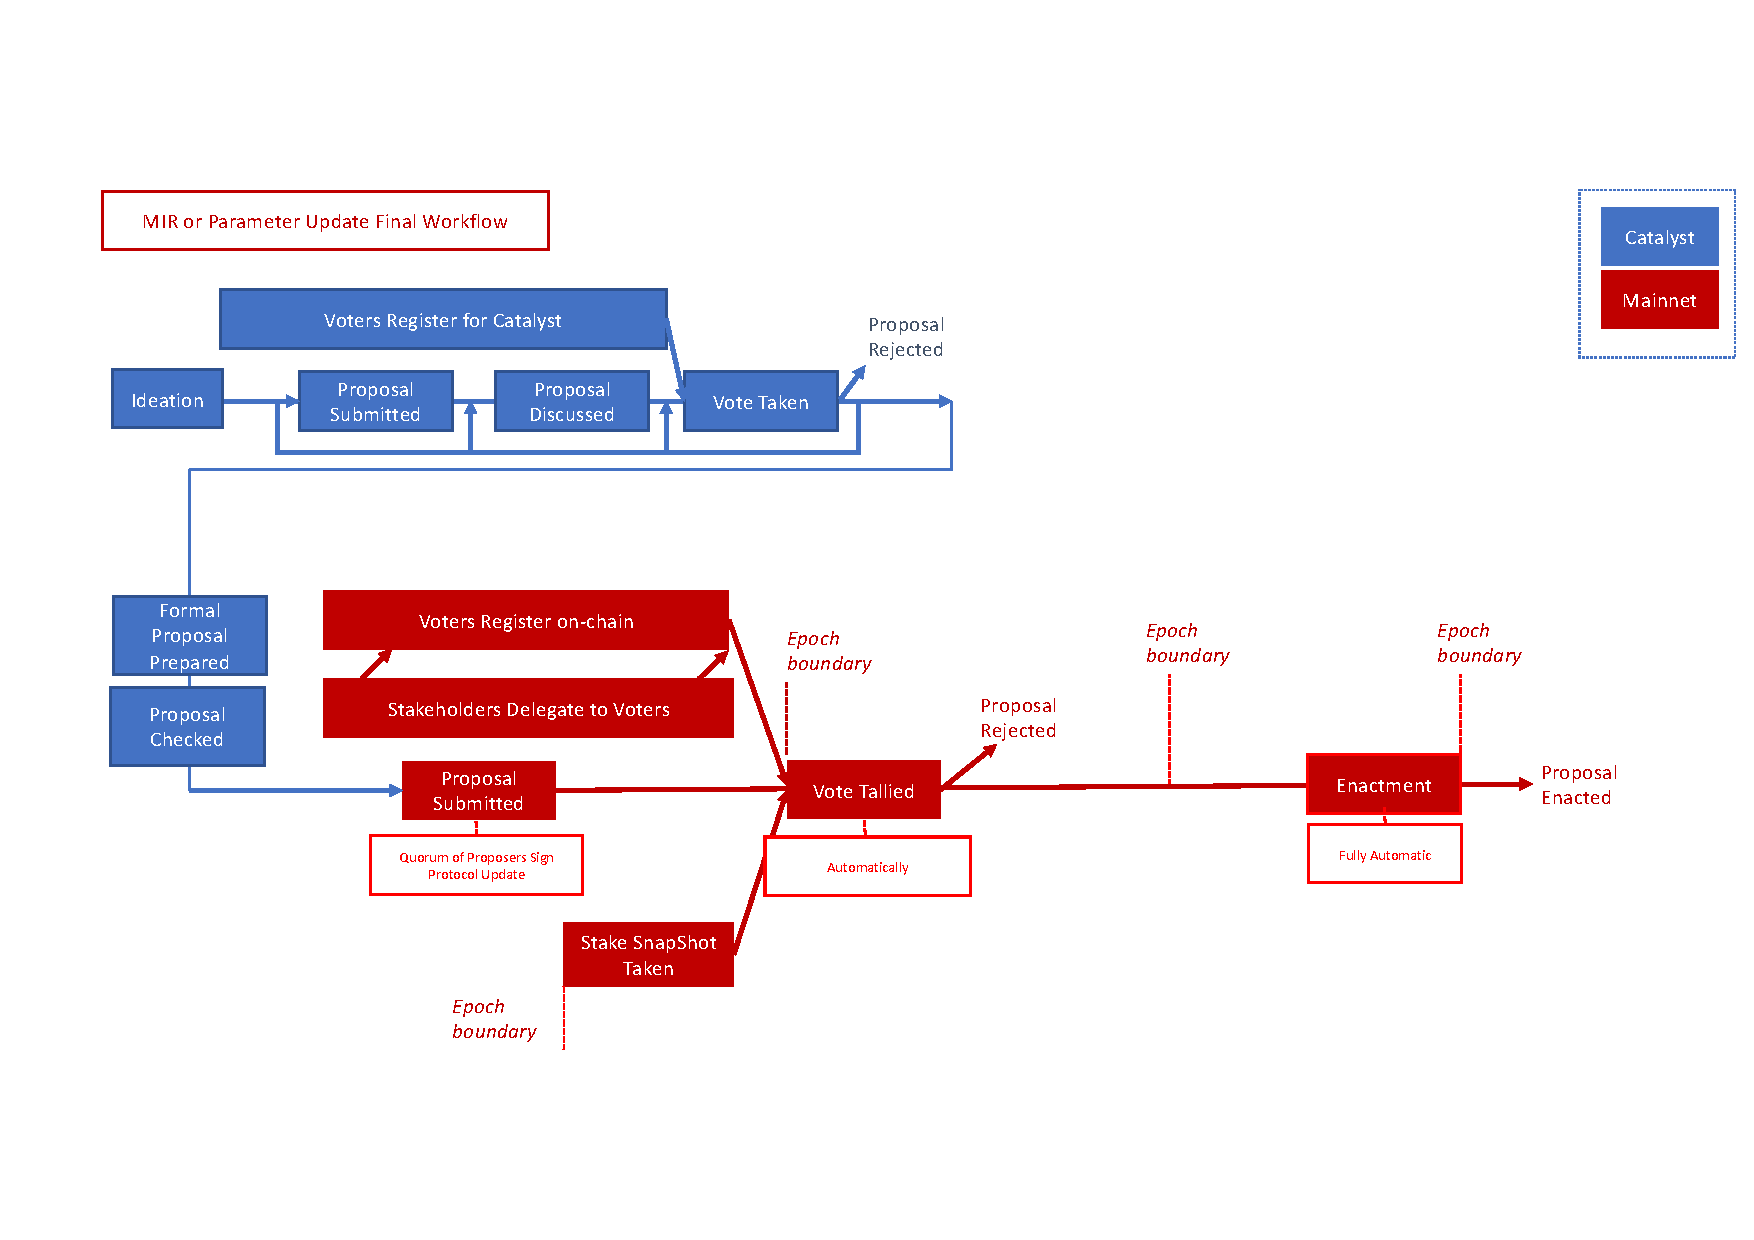
\includegraphics[angle=270,trim=0 90 0 90,clip,width=0.7\textwidth]{Workflow3}
%  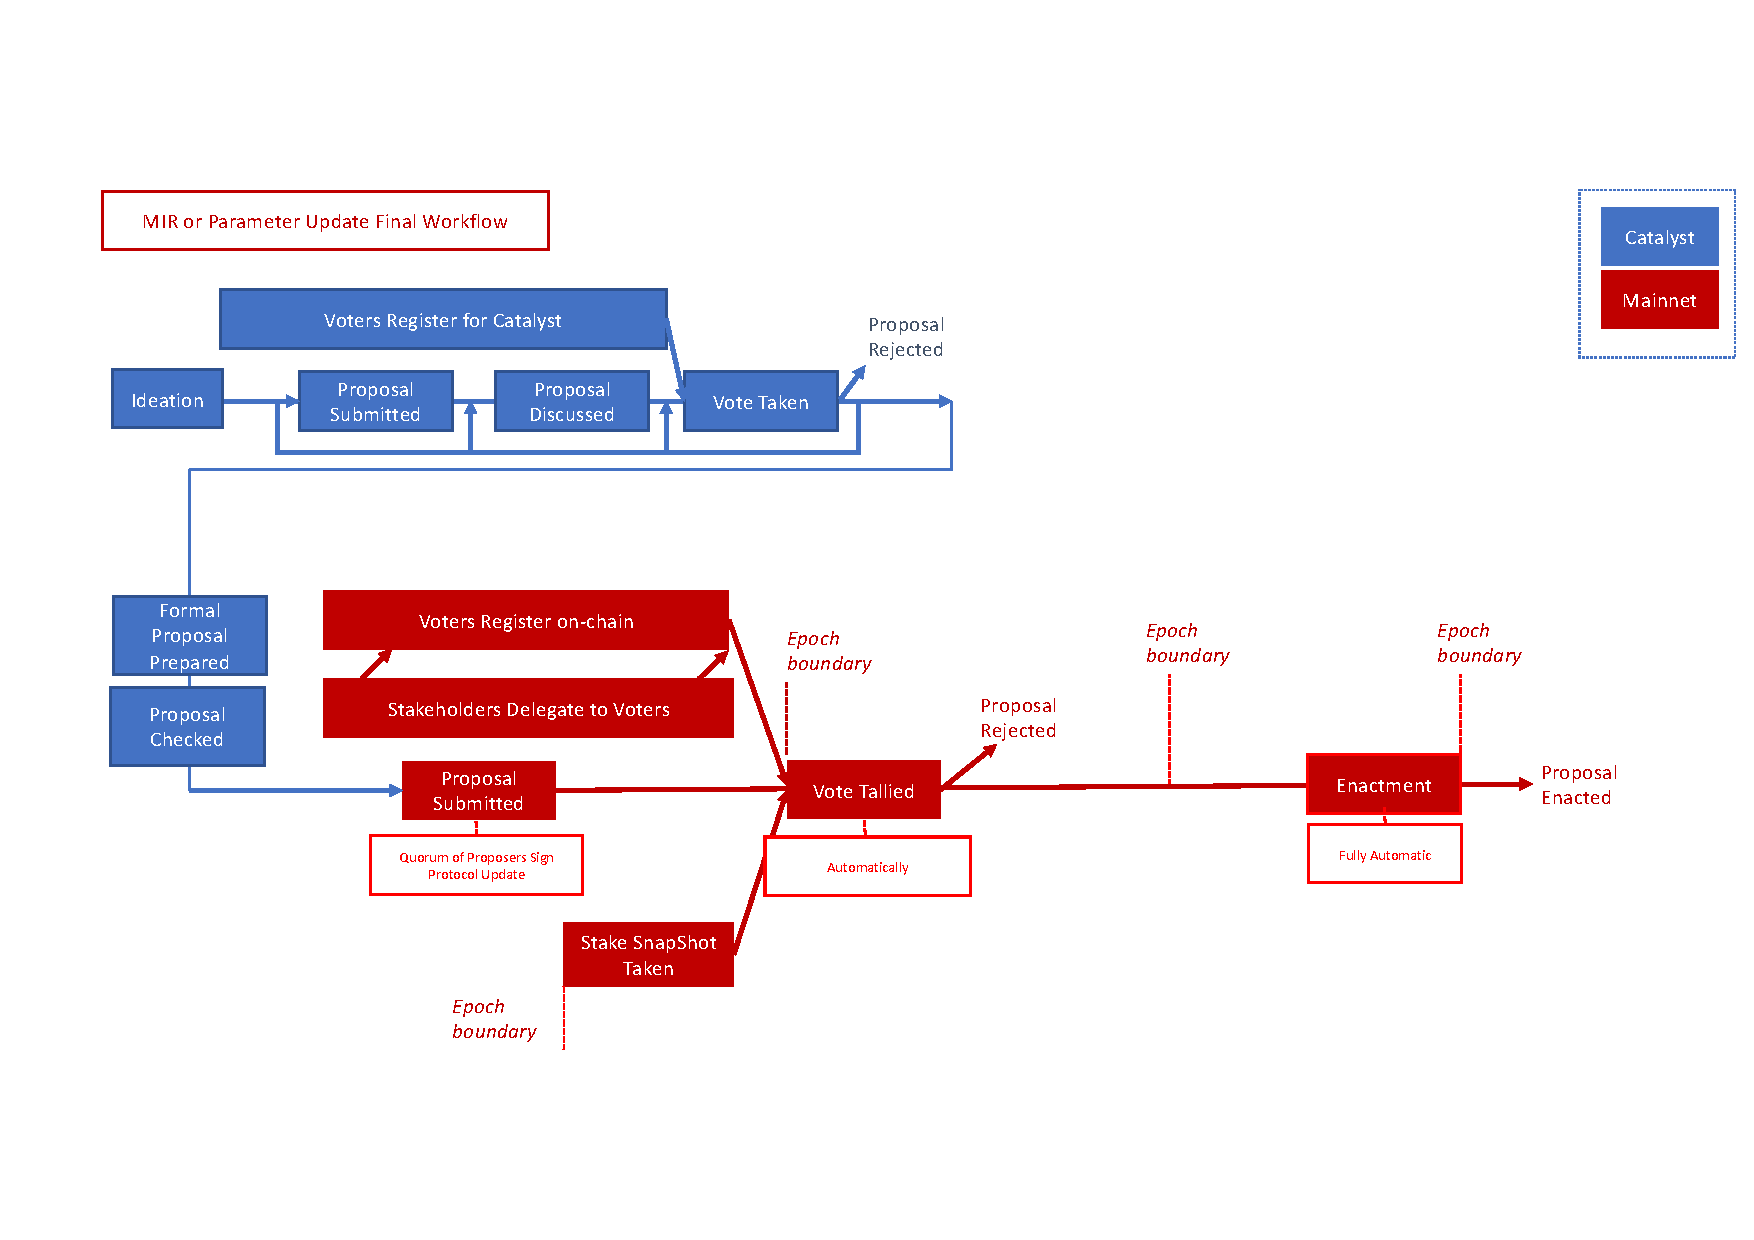
\includegraphics[trim=0 90 0 80,clip,width=\textwidth]{Workflow3}
  \caption{Example Workflow: Funds Transfer (MIR) or Simple Parameter Value Update, showing off-chain delegation and voting simulation steps for initial pilot}
  \label{fig:workflow-mir2}
\end{figure}

\begin{figure}
  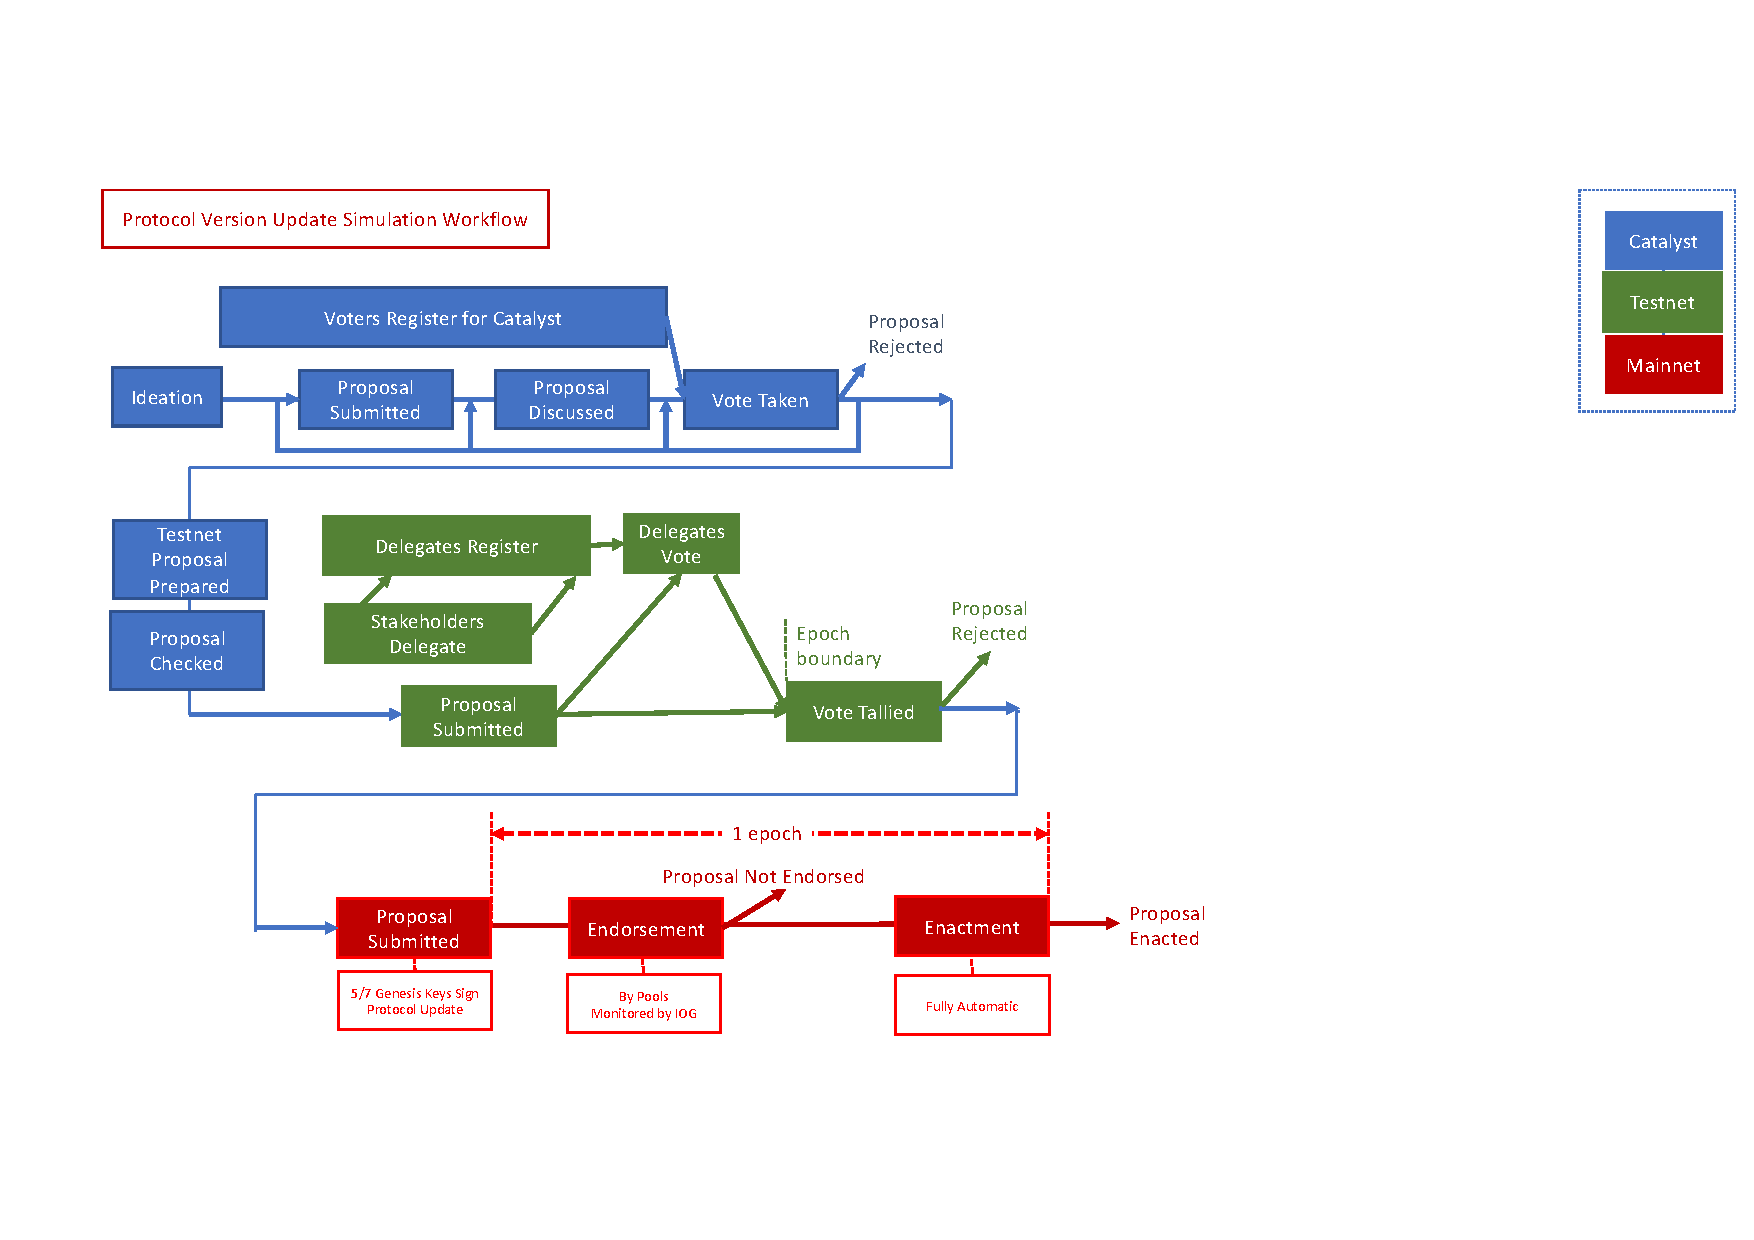
\includegraphics[angle=270,trim=0 90 0 90,clip,width=0.7\textwidth]{Workflow4}
%  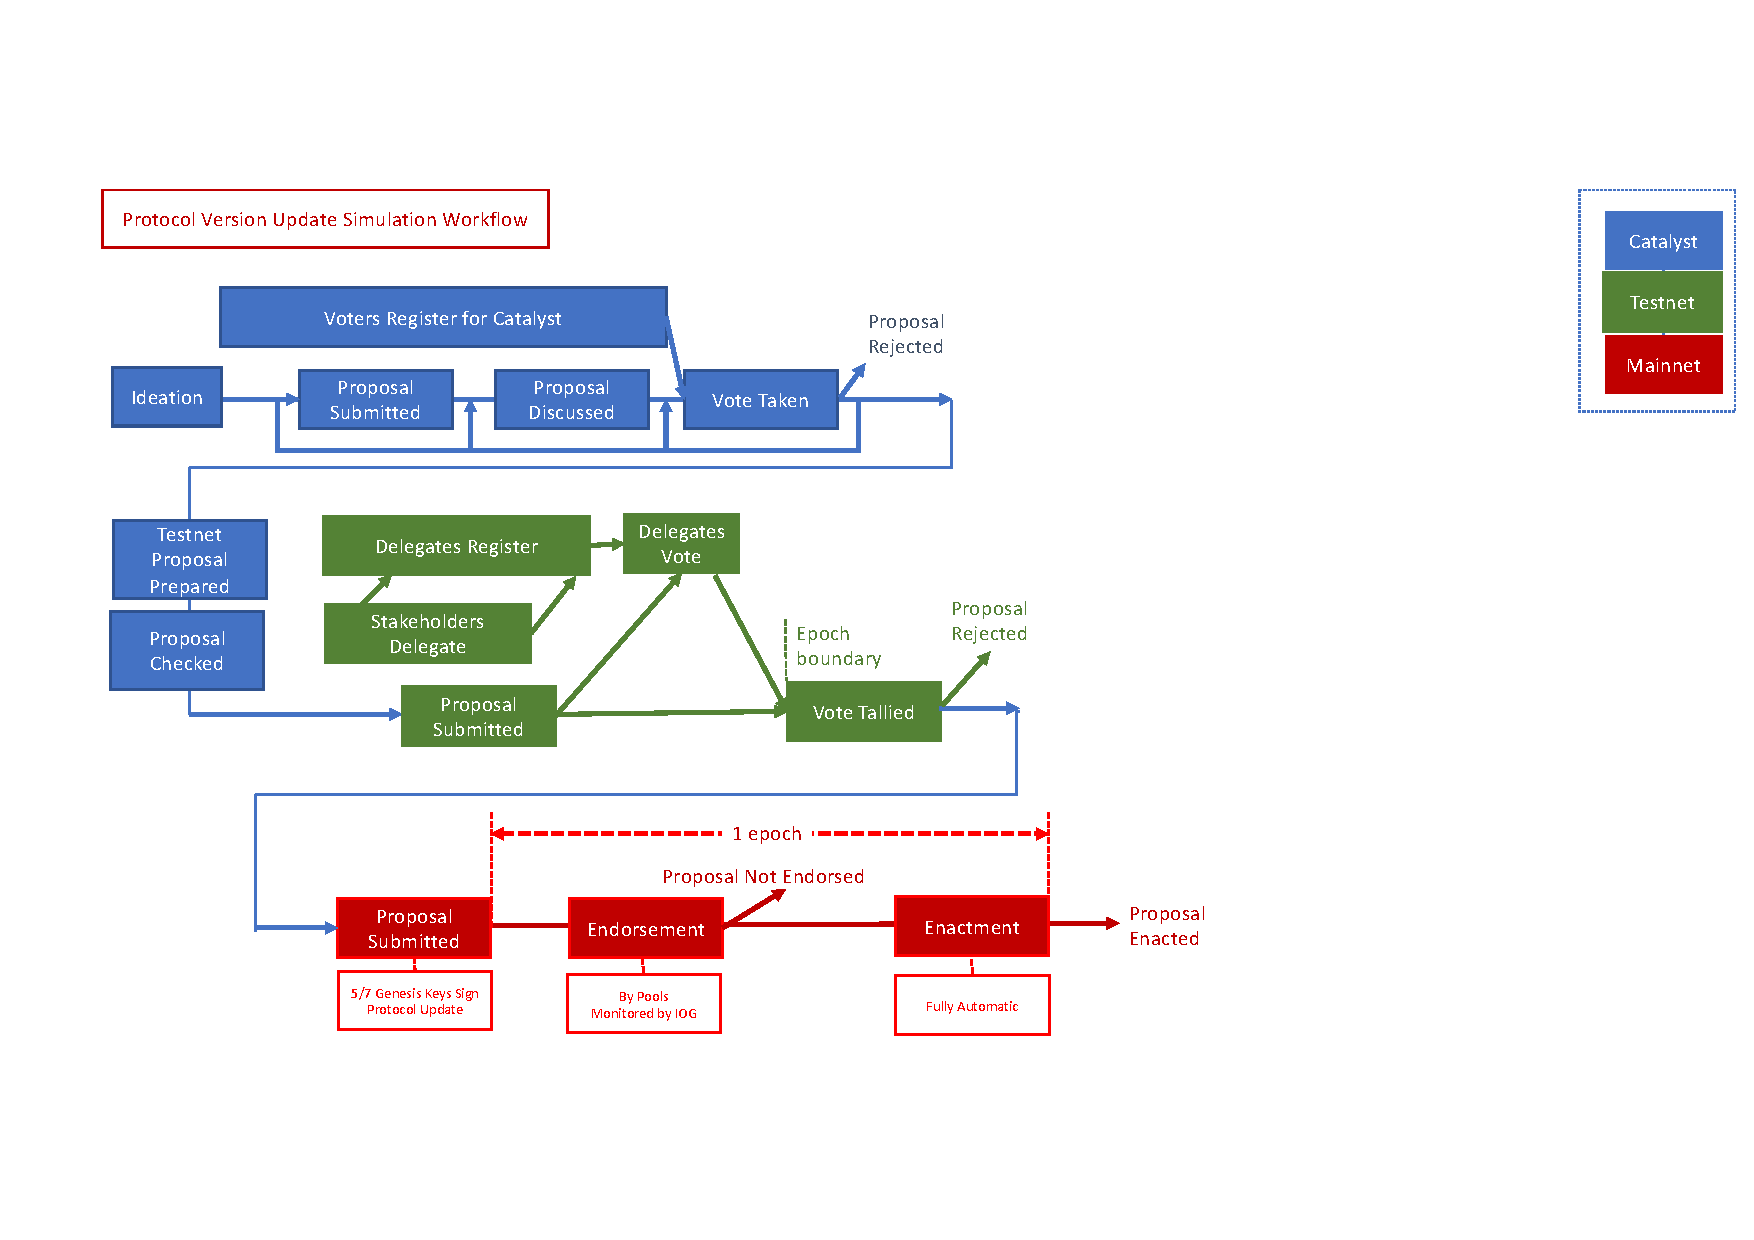
\includegraphics[trim=0 90 0 80,clip,width=\textwidth]{Workflow4}
  \caption{Example Workflow: Protocol Version Update (Hard Fork), showing off-chain delegation and voting simulation steps for initial pilot}
  \label{fig:workflow-hf2}
\end{figure}

\subsection{Workflows for Accelerating Early Governance Pilots.}
\label{sect:pilot-workflows}

Figures~\ref{fig:workflow-mir2}-\ref{fig:workflow-hf2} show the corresponding  workflows that could be used if desired,
for initial pilots.  The off-chain process is identical in all cases, but the on-chain delegation process is mimicked precisely on a testnet, rather than performed
on-chain.  Accepted proposals are then passed for manual submission and enactment on-chain.  This will allows early testing and tuning of governance mechanisms without
irrevocably changing the on-chain governance process, so permitting more rapid deployment of decentralised governance with reduced implementation and automation risk.

\subsection{Genesis Keys/Genesis Delegates}

Once the protocol has been updated to include the on-chain PUP mechanisms, the
genesis keys and their delegates will cease to have any governance power.  The
chain can only legitimately be continued through the decentralised governance
mechanism.  Once the chain has been extended, and it is decided that the chain
will never need to be reverted, the keys may safely be destroyed.


\clearpage
\pagebreak
\section{User Experience}
\label{sect:ux}

This appendix outlines how the voting experience could appear to ada holders and other user groups.

\subsection{General Ada Holder Experience}

\paragraph{General Process.} An ada holder registers their account in the voting centre.  As a result, they obtain both Catalyst voting rights and on-chan vote delegation rights.
The voting centre displays a list of registered delegates, and allows them to delegate their vote to any delegate that they choose.  Transaction
fees are paid for registration and for vote delegation.  The ada holder may choose to participate in the off-chain discussion and voting process for any
parameter update or funds transfer. They will receive ada rewards for their participation.
Voting rights are proportional to the ada that is held, both in Catalyst and on-chain.  However, there may be lag in the Catalyst system.\khcomment{It would be possible to export the vote snapshot at each epoch,
  so that the Catalyst system could be kept up to date.  At present, the stake transfer is manual and uses a \texttt{db-sync} snapshot -- this would need to be automated, and there might need to be some changes to the Jormungandr system
  so that it could easily record dynamic stake changes.  Token locking information might also need to be recorded.}

\paragraph{Catalyst Process.}

This needs to be defined, but in essence:

\begin{itemize}
\item
  Ada holders register for Catalyst voting through the voting centre;
\item
  Voters are informed of active proposals in areas that interest them;
  \khcomment{There is a tension here between participation and overload -- ada holders may find parameter updates to be too technical, for example}
\item
  Using the Catalyst vote mechanism, ada holders vote on whether the proposal should be accepted, rejected or revised -- there may be multiple voting rounds
  before a decision is finalised;
  \khcomment{This may reflect a change in the current Catalyst process?}
\item
  Once a proposal is accepted, it proceeds to formal implementation and on-chain enactment.
\end{itemize}

\paragraph{On-Chain Vote Delegation.}

Ada holders may delegate their on-chain vote whenever they choose.  Vote delegation may be changed at any point in time through the voting centre, in
exactly the same way as stake pool delegation.  Ada holders are warned if their chosen delegate announces their retirement, and may then redelegate their vote if they
wish.  If they do not redelegate their vote, it will not count towards any future decision.\khcomment{Note the different possible voting thresholds.}
When an ada holder withdraws their ada holding, they will lose their voting rights with effect from the next stake snapshot (i.e. at the start of the next
epoch).  Similarly, when they acquire ada, they will acquire new voting rights with effect from the next stake snapshot.
Ada holders may track how their delegates have voted on-chain, and may reassign their vote delegation if they wish.

\subsection{Delegate Experience}

Ada holders may choose to become vote delegates.  They may do this on their own behalf, or as public delegates that act as proxies for other ada holders.
Public delegates will be influential community members, with public duties and responsibilities.
A delegate first registers themselves in the voting centre.  As public delegates, they may then advertise their voting intentions to other ada holders and canvas for vote delegations.
They will participate in and follow discussions about proposals in various forums, track on-line proposal submissions, and
record their vote for each proposal before the stated deadline using the voting centre.  They may track the outcome of each proposal using the proposal explorer, and inform their
delegators of the proposal outcome.
\khcomment{It is not obvious what motivates delegates to participate? They have duties and responsibilities.}

\subsection{New Tools/Mechanisms to Support the User Experience}

A number of new tools or mechananisms are needed to support the user experience:

\begin{enumerate}
\item
  A way to prepare business for discussion and voting via Catalyst;
\item
  A way to track proposals -- this implies either a significant extension to the voting centre, or some new ``proposal explorer'' capability;
\item
  Changes to the voting centre to support on-chain vote registration, vote delegation etc.;
\item
  A way for delegates to register and to record their on-chain votes -- perhaps via the voting centre, or perhaps via CLI commands;
\item
  A way for delegates to make themselves known to potential delegators;
\item
  A way for ada holders to become aware of delegates, including the number of votes that they control.
\end{enumerate}

% All of these mechanisms will need to be designed and implemented.

Proposal submission and endorsement will be done by technical experts, so can be handled via CLI commands.  It may be reasonable for delegates
to also use the CLI, but they may have less technical expertise than stake pool operators, for example.

\paragraph{Tracking Proposals.}

An explorer or other mechanism needs to be set up so that the status and progress of proposals can be tracked by stakeholders.  A single off-chain proposal may give rise
to multiple on-chain proposals that need to be linked to the original proposal.  Section~\ref{sect:proposalid} describes some ways that proposals may be identified, and used
to link off-chain and on-chain proposals.


\clearpage
\section{Tracking Proposals through a Side-Chain}

It has been suggested that a specific proposal could be submitted on-chain, with voting on the proposal tracked through a side-chain, such as Catalyst.
While it is probably not sensible to include this in the initial design, since it would add complexity and delay implementation, a system such as this
may be worth considering in future.

\subsection*{Main Advantages.}

\begin{tabular}{||l|p{4.5in}||}
  \hline\hline
  Reuse
  & Side-chain mechanisms are already being developed for other purposes (Hydra), so it might be possible to reuse existing design/implementation work.
  \\ \hline
  Automated Submission
  & A proposal could be submitted automatically on-chain, once a vote was accepted.
  \\ \hline
  Automated Tracking
  & The evolution of a proposal could be tracked automatically.
  \\ \hline
  \hline
\end{tabular}

\subsection*{Main Disadvantages.}

\begin{tabular}{||l|p{4.5in}||}
  \hline\hline
  Additional Work/Risk &
  Tracking the vote on a proposal correctly could require significant work to be completed on side-chain integration, so delaying the project as a whole.
  \\\hline
  Fit with Catalyst &
  The intention is to use Catalyst for voting, so the mechanism must integrate with the Catalyst chain.
  \\\hline
  Implementation Timing & A proposal will typically only be crystallised into a form that can be submitted on-chain (implemented) \emph{after} it has been approved by an off-chain vote.
  This can involve a significant amount of work and perhaps financial support.
  It is important that any system that tracks the progress a proposal through a side-chain does not require it to be crystallised before it has been approved for implementation.
  \\ \hline
  \hline
\end{tabular}

Changes to side-chain proposal tracking could affect the on-chain submission process, but should have no impact on the remainder of the on-chain process.


\clearpage
\section{Comparison with the approach taken by the Priviledge Project}

The key differences between the mechanism and that produced for the EU Priviledge project are:

\begin{tabular}{||p{3in}|p{3in}||}
  \hline\hline
  \textbf{Priviledge} & \textbf{PUP}
  \\\hline
  Completely on-chain & Uses Catalyst as well as on-chain \\\hline
  Supports vote abstention & Treats abstention as rejection \\\hline
  Allows multiple voting rounds & Allows only one round on-chain \\\hline
  Allows arbitrary vote stake snapshots & Takes vote snapshots at fixed points \\\hline
  Allows explicit prioritisation & Time-based prioritisation \\\hline
  Does not restrict submission & Restricts submission \\\hline
  Includes software upgrades & Does not consider software upgrades \\\hline
  Does not handle funds transfers & Handles central funds transfers \\\hline
  Does not support vote delegation & Supports vote delegation \\\hline
  Includes version number for upgrades & No version number \\\hline
  Does not include specific protocol parameters & Includes protocol parameter updates \\\hline
  \hline
\end{tabular}

\khcomment{First draft.  Each of these points could be expanded on, if required.}


\clearpage
\pagebreak
\section{Extensions to Enable Governance for Native Tokens}
\label{sect:native-tokens}

This appendix considers how these mechanisms could potentially be extended to enable
governance mechanisms for native tokens, for example to govern the supply of specific tokens.
Major changes might be needed compared with the general PUP system.  These issues are discussed below.

\subsection{Integration with Off-Chain Mechanisms}

Any desired mechanism, including informal ones or side-chains, could be used to initiate ideation and discussion or for
initial voting.  This might include Catalyst, provided that a suitable way to obtain snapshots could be devised.
A purely on-chain mechanism would probably be sufficient for most native tokens governance, however.

\subsection{Proposals}

The proposal submission mechanism would need to be adapted for native tokens.

\begin{itemize}
\item
  Proposals would need to be restricted to the correct native token.  This could be done by embedding the monetary policy script hash in the proposal.
\item
  Proposals would be restricted to relevant governance issues rather than protocol parameters, protocol updates or central funds transfers.
  These issues could include:
  \begin{inparaenum}
  \item
    parameter settings related to the monetary policy script (which could be a smart script once Plutus core is deployed);
  \item
    decisions on increasing/reducing the supply of one or more tokens;
  \item
    decisions on transferring tokens to specific accounts (e.g. a ``treasury'');
  \item
    decisions on who can authorise the minting or burning of new tokens (and, of what types), including new signing policies (if this is possible in future);
  \item
    decisions on whether to issue new tokens.
  \end{inparaenum}
\item
  Proposals would need to be signed by a quorum of submitters.  The obvious approach is to use the minting policy script.
\end{itemize}


\subsection{Voter Registration}

Since native tokens are always associated with UTxOs, the same vote key
registration mechanism could be used as for Cardano.  There might be no need to
register for each different kind of native token.  However, such an approach
would only allow one delegation from each address (so the same delegation would
cover Cardano and native tokens votes), which could create
confusion/opportunities for subversion.  A solution might be to hold native
tokens separately from large ada holdings, so creating granular voting rights.
The alternative of allowing multiple voter registrations potentially creates
clutter, and may require some internal fields to be arbitrary sized.

\subsection{Vote Delegation}

The standard delegate system might be overly complicated for most native tokens.
However, voters could register as delegates so that they could cast their votes
directly.  This would carry some fee for the registration and vote transactions.
Alternatively, the token issuer could register standard Yes/No delegates, and
ensure that these always voted in the required way.  A voting centre could hide
the complexities of delegate registration.  Care would need to be taken to
distinguish delegates for Cardano and non-Cardano purposes.  Conceivably, a
single delegate could vote for different native tokens on behalf of a single
token holder.

\subsection{Snapshots, Tallies and Thresholds}

\paragraph{Snapshots.}
Unlike ada, native tokens can be minted or burnt at any point in time, meaning
that the token supply for any native token could fluctuate significantly.  At
present, the total circulation of each native token is never calculated.
Real-time circulation calculations in the ledger are probably not practical from
an efficiency (and therefore security) perspective.  The simplest solution would
be to take voting snapshots for native tokens at the same time as for ada (at
each epoch boundary).

\paragraph{Circulation.}
Native tokens will typically be minted en-masse, and then issued piecemeal.
This needs to be considered in calculating the total supply and voting
thresholds for each token.  Tokens that are held by the token issuer and have
never been issued should probably not count towards the circulation (they are
equivalent to the Cardano reserve).  Similarly tokens that have been returned to
the issuer should not be counted in the circulation, even if they have not been
burnt (they have been returned to the reserve).  Finally, tokens might be held
within special-purpose accounts (e.g. as the equivalent of the Cardano
treasury), and should not be counted towards circulation.  This implies either
imposing some structure on token accounts, or else providing customisable rules for
each asset class.

\paragraph{Performance Issues.}
One major issue that must be addressed is the need to maintain multiple voting
credential maps (one for each native token).  This could have significant memory
implications as well as increased execution time.  In order to avoid slow-downs,
it might be necessary to create/update credential maps incrementally (e.g. when
tokens were issued/transferred/burnt).

\paragraph{Differential  Voting Rights.}
Different kinds of tokens may have different voting rights.  For example, a
currency might have Class A and Class B tokens, where Class A tokens have full
voting rights and Class B tokens have partial or no voting rights.  This could
create complications in calculating voting thresholds.  One solution might be to
separate tokens into different asset class, where a vote on one asset class
could govern decisions on another asset class.  So Class A tokens might be able
to take governance decisions on Class B, but not vice-versa, for example.
Similar considerations apply to Non-Fungible Tokens, adding specific kinds of
value to these tokens.

\paragraph{Thresholds.}
Unlike Cardano, there is no need to set minimum voting thresholds.  These can be
set on each proposal as required.

\subsection{Endorsement.}

Since native tokens cannot affect the Cardano protocol itself, there is no need for an endorsement mechanism
for native token proposals.

\subsection{Automated Enactment.}

Automated enactment might be implemented by calling suitable Plutus smart contracts, for example.  Unlike
Cardano, it is not necessary for automated enactment to be tied to an epoch boundary.


\clearpage
\pagebreak
\section{Expert Ballots}
\label{sect:expert-ballots}

This appendix considers how ``expert ballots'' could be integrated into the on-chain enactment process.
An expert ballot is a manifesto by a group of experts that presents an easily understood voting intention
(or collected group of intentions).  Under the assumption that it is not necessary to consider each issue
independently (which might place significant load on ada holders in assessing the quality of each ballot on
a regular basis), the PUP approach fits such an approach well.

\subsection{Proposal Submission}

No changes are needed to the proposal submission process.  Expert groups will monitor the progress of proposals
and update their expert ballots in advance of voting (perhaps even in advance of submission).

\subsection{Vote Delegation}

The delegate mechanism described here can be used to directly support expert
ballots.  Expert groups may register as delegates, and ada holders may choose to
delegate their vote to those groups either on a per-issue basis or over a period
of time.  As usual, Ada holders may change their voting intention at any point in time.
This flexible approach will suit enterprise ada holders (where it may take substantial
effort to change a set of vote delegations) as well as individuals (who may

\subsection{Endorsement and Enactment}

No changes are needed to the endorsement and enactment phases.  Protocol version updates will need
to be endorsed by block producers, and enactment can be carried out automatically.


\subsection{Voting Centre}

The voting centre would need to be changed so that expert ballots could be presented to ada holders,
and so that vote delegations could then be made to these expert groups.  Users might also want
to be alerted to new ballots (perhaps filtered in some way).

For example, a user might be presented with an expert ballot, given the opportunity to read the ballot
and conduct any background research, and then reject the ballot, select it as a voting choice, or
save it for later consideration.


\clearpage
\section{Possible Extension to Differentiated Submitter Groups}

This design assumes a single group of submitters.  It
would instead be possible to differentiate proposals, so that specific kinds of proposal
could be submitted by different sub-groups.  For example, a sub-group of submitters might have
authority to submit a proposal that changed specific parameters, that authorised
funds transfers up to some amount, that transferred balances between reserves
and treasury, or between treasury and specific nominated accounts.  The obvious
way to do this would be to embed general Plutus scripts in the submission
authorisation (or to allow Plutus scripts to construct proposals).  This could
involve some changes to ledger rules (including perhaps changes to script
plumbing), so should probably be seen as an extension to the base design, rather
than a core requirement.  \todo{Consider whether a script can be used for
  proposal submission rather than embedded signatures.  Does the two-phase Plutus process cause unwanted delays?}

For such an approach to be feasible, it would be necessary to determine whether
a proposal was permitted to be signed by a specific sub-group (i.e. the proposal
would need to be automatically checked and validated against the group
credentials).  It would also be necessary to set thresholds and quora
differently for different kinds of proposal.  These thresholds would need to be
independently validated through security audit.


\clearpage
\section{Security Audit Reports}

\subsection{Report from BCryptic: 2021-05-03}

% \VerbatimInput{security-reviews/2021-05-03.rtf}


\definecolor{color02}{rgb}{0.98,0.01,0.03}
\definecolor{color03}{rgb}{0.98,0.01,0.03}


\textbf{Review of The Design of the Cardano Ledger with Automated Parameter Updates 
and Central Fund Transfers (April 30, 2021 version)}

\vspace{12pt}
\begin{center}
\textbf{Possible Current Issues: }
\end{center}

\vspace{12pt}
\baselineskip=12pt
\leftskip=0pt
- Some questions about stake snapshot versus vote delegation: p19, Fig 2: In the 
figure, the snapshot of the stake distribution is concurrent to the delegates voting. 
However, in the real execution the snapshot must be before the voting, right? Or 
else how could pools that are making blocks know whether a vote is valid and should 
be included in a block? From p30, Fig 7 the snapshot is before voting, which makes 
sense. However two questions:

\parindent=18pt
(1) Can delegations change during vote casting time, or once voting period begins 
delegation changes do not count? From Fig 7 it seems the latter is true. However, 
in Section 7.3 (Tallying Votes) it says ``total vote... is the sum of all active 
delegations at the point that the vote is tallied'', which feels it implies the 
former.

\vspace{12pt}
\parindent=0pt
{\color{color02} Delegations and vote choices can change at any time prior to the 
vote deadline.  We will adjust Figure 7.}

\vspace{12pt}
\parindent=18pt
(2) There may be edge cases to consider. For example: Suppose at the time of the 
stake snapshot I have some ada. However, after the snapshot I sell my ada. Should 
I still be able to redelegate my vote?

\vspace{12pt}
\parindent=0pt
{\color{color03} This is inevitable with a snapshot approach.  Likewise not being 
able to vote immediately that ada is acquired.  It is, of course, consistent with 
block production (I can earn rewards after I have sold my ada), so carries no greater 
risk.  The alternative (compute a snapshot for each vote) would be very inefficient 
(repeated snapshotting, which we need to avoid if possible), and also leads to 
``buy significant ada, vote, sell ada''.  Token locking helps solve that, but reduces 
participation, which is highly undesirable (and could reduce security/lead to lack 
of progress, depending on how totals were calculated).  Overall, the edge cases 
are likely to be minor, with less serious consequences than the alternative.}

\vspace{12pt}
- p23, Option 3 (transaction identifier is used to identify the proposal): This 
can be dangerous, since the location the proposal ends up on chain is not fixed 
until it is part of common prefix. If there are multiple concurrent proposals this 
can lead to people accidentally voting for the wrong proposal (or worse, malicious 
pools can exploit this for their advantage).

\vspace{12pt}
{\color{color02} Noted.   It would be unlikely, of course, but the proposal contains 
additional information that tie to a specific set of actions, so this could be 
hashed, for example.}

{\color{color02} Pools don't vote, but delegates could be malicious.}

\vspace{12pt}
- Section 8 and 9: It is not very clear right now whether multiple protocol version 
changes can happen in a single epoch.

\parindent=18pt
(1) Might there be issues if this can happen?

\vspace{12pt}
\parindent=0pt
{\color{color02} Only one could be adopted (the change can only be one Hamming 
distance from the current protocol version).  All minor version changes are equivalent, 
as are all major version changes,}

{\color{color02} so the only possible ambiguity comes where there is a conflict 
between a major and a minor upgrade.  The current design resolves this mechanically 
through temporal ordering, but an alternative would be for eg a major upgrade to 
override a minor upgrade (in which case the minor upgrade would never happen).}

\vspace{12pt}
\parindent=18pt
(2) If it can happen, Section 9.2 which says ``multiple update proposals...are 
enacted strictly in the order that they were submitted'' should also include ``and 
enacted in the order of the protocol version for protocol version changes''.

\vspace{12pt}
\parindent=0pt
{\color{color02} That is not necessary.  See above.  It probably also doesn't work 
technically (AFAIK, the hard fork combinator will only process one upgrade at an 
epoch boundary --- I will check its semantics!).}

\vspace{24pt}
\begin{center}
\textbf{Security concerns:}
\end{center}

\vspace{12pt}
\baselineskip=12pt
\leftskip=0pt
- p14, ``resolve conflicts between proposals automatically'' - There should be 
a lot of care taken when going this route, since a voter can vote for one proposal 
A without knowledge about another proposal B. The two proposals might not even 
conflict, but just not synergise well. For example, if A reduces the max size of 
a block and B increases the max size of a transaction, then together they may cause 
undesirable consequences (e.g. too few transactions allowed in a block).

\parindent=18pt
-\texttt{>} Perhaps a way to combat this is allow a proposal to declare a ``conflict 
set'', e.g. a proposal A is not compatible with another proposal B, if B modifies 
parameter x. 

\vspace{12pt}
\parindent=0pt
{\color{color02} This solution would require knowledge of all other proposals (which 
would be impractical), and would only work for a rational/honest submitter set. 
 If we assume a rational/honest submitter group, however, then we can assume that}

{\color{color02} they will anyway have resolved the conflict, in which case this 
is not really necessary.  The only solution I can envisage is to automatically 
check for inconsistencies, but that is difficult to achieve with the current parameter 
design (you would perhaps need logical constraints on each parameter to define 
possible conflicts).  Or we can rely on rational/honest voters to detect possible 
conflicts.}

\vspace{12pt}
\parindent=18pt
-\texttt{>} Another thing to be careful about is that temporal orderings might 
not be reliable, since the order of blocks can be (at least slightly) influenced 
by malicious parties.

\vspace{12pt}
\parindent=0pt
{\color{color02} Noted.  We can assume that the submitter group is honest and aware 
of possible malicious influence.}

\vspace{12pt}
- p15, Security Requirements: Another issue that would be good to address is that 
it seems stake pools have a big power over voting. For example, suppose there is 
a proposal that is desirable for normal users of the system, except many stake 
pools do not like this proposal. Then, it may be possible for these stake pools 
to ensure that this proposal is never put onto the blockchain, or at least delay 
this proposal until e.g. the vote deadline. 

\parindent=18pt
-\texttt{>}  Of course, by the security assumption, honest stake pools will include 
even proposals they do not like, but this may not be the case for rational stake 
pools.

\vspace{12pt}
\parindent=0pt
{\color{color02} To be clear, stake pools endorse, but don't vote or submit proposals. 
 The vote and endorsement deadlines are absolute, so there can be no delay (a proposal 
is either accepted at the deadline or it is not - everything else is irrelevant).}

{\color{color02} Endorsement is limited to protocol upgrades, so pools have no 
direct control over parameter updates - submitters and delegators have all the 
power.  }

\vspace{12pt}
{\color{color02} A pool that doesn't endorse a protocol upgrade will become disconnected 
from the main chain.  So it's important to avoid chain splits that sufficient pools 
endorse a proposal (as defined by the endorsement threshold).  }

{\color{color02} There is no way to force a pool to upgrade.  So yes, they do collectively 
have power of veto on protocol upgrades.  That is seen as reasonable - they bear 
the cost of maintaining the network}

{\color{color02} and have technical knowledge of the impact of an upgrade.  However, 
if the upgrade was in the interest of the chain, and stakeholders agreed on this, 
they could choose to re-delegate their stake}

{\color{color02} to pools that would upgrade (even forming new pools).  So no group 
of pools could postpone an honest upgrade indefinitely (even 100\% ``dishonesty'' 
can be overcome by forming new pools).}

\vspace{12pt}
{\color{color02} In practice, pools are unlikely to oppose an upgrade unless there 
are technical issues with it.}

\vspace{12pt}
- p18, Submitters: For decentralisation it is important to ensure that submitters 
is not restricted to too few members.

\vspace{12pt}
{\color{color02} Noted and agreed.  There will be a practical limit on numbers 
(how many signatures can be included in a transaction), but this will be around 
200-400.}

{\color{color02} There is a requirement to limit the size of the submitter group 
to avoid ``flooding'' (a denial of service where honest proposals are swamped by 
dishonest ones, so voters are overwhelmed by choice/cost).}

\vspace{12pt}
- p22, ``Central Funds Transfer Body'' - Since there is no UTxO with the treasury/reserves, 
one must be careful about accounting to avoid double-spending. 

\vspace{12pt}
{\color{color02} Noted.  There are existing formal accounting rules/properties 
that are followed for manual funds transfers, including overall preservation of 
ada.  These need to be preserved.}

\vspace{12pt}
- p23, comment on using multisig for submitter signing: Depending on the size of 
the submitter group, one must be careful about the signatures not exceeding max 
transaction size.

\vspace{12pt}
{\color{color02} Yes.  This limits the number of signatories.  The same issue applies 
to a specialised proposal format.}

\vspace{24pt}
\begin{center}
\textbf{Questions/Comments/Suggestions:}
\end{center}

\vspace{12pt}
\baselineskip=12pt
\leftskip=0pt
- p12, section 1.4 - Here can also say that exchanges/proxy holders can declare 
themselves as not holding any stake (their address should clearly indicate this)

\vspace{12pt}
{\color{color02} At present they don't.  There is an address format for this purpose, 
but it is unused, and cannot be enforced.}

\vspace{12pt}
- p21, the comment on submitters being trustworthy: Perhaps we can use a similar 
method to choosing slot leaders to choose the submitters, so we use the same assumption 
of honest majority of stake as the cryptographic security.

\vspace{12pt}
{\color{color02} Full randomness doesn't work for this purpose.  A submitter has 
to be prepared to submit a proposal, to collate counter-signatures, and to pay 
any fees.}

\vspace{12pt}
- p21, the comment on setting minimal thresholds for vote enactment''. I agree 
there must be some kind of limit of how low a vote threshold can be, or else there 
could be proposals that are enacted even if very few people voted on it. An idea 
is to require that a proposal must *both* (1) have a number of ``yes'' votes that 
is above the vote threshold, and (2) have a number of ``no'' votes that is lower 
than the vote threshold. This means a proposal with low threshold can be outvoted 
if a problem is found with it, and also makes use of the ``no'' vote (by Section 
7.1, at the moment, there is no point of casting a ``no'' vote as this is the same 
as not voting.

\vspace{12pt}
- p23, comment on collision resistance: Yes, collision resistance is required.

\vspace{12pt}
{\color{color02} Thank you.}

\vspace{12pt}
- p25, the ``Confirm.'' and ``Confirm this.'' comments: Should be ``yes'' to both.

\vspace{12pt}
{\color{color02} Thank you.}

\vspace{12pt}
- p31, comment on recording the tally on chain: Yes, I believe it could be good 
for performance, similar to recording the result of scripts.

\vspace{12pt}
{\color{color02} Thank you.  We will note this.}

\vspace{12pt}
\begin{center}
\textbf{Typos/Minor:}
\end{center}

\baselineskip=12pt
\leftskip=0pt
{\color{color02} Thank you. We will apply these.}

\vspace{12pt}
- p4 ``There c'' (unfinished sentence)

\vspace{12pt}
- p9 ``nomrmal'' -\texttt{>} ``normal''

\vspace{12pt}
- p19 ``where the proposed...'' -\texttt{>} ``where the proposal...''

\vspace{12pt}
- p23 ``All update'' -\texttt{>} ``All updates''

\vspace{12pt}
- p27 Missing citation at ``...from the Shelley delegation design document...''

\vspace{12pt}
- p28 ``...refer to a vote credential that is must be...'' -\texttt{>} ``refer 
to a vote credential that must be...''

\vspace{12pt}
- p28 Missing citation at ``...stake address references (see ?)...''

\vspace{12pt}
- p34 Missing citation in Section 9.1 after ``hard fork combinator''

\vspace{12pt}
- p35 Missing descriptions in table

\vspace{12pt}
- p36 ``prpgress'' -\texttt{>} ``progress''

\newpage



\end{document}
